% Preamble {{{1
% There's some issue that causes captions like "Listing 2.: Foo".  setting the `numbers`
% option like this fixes it.  See <https://tex.stackexchange.com/q/29181>.
\documentclass[a4paper,numbers=noenddot]{scrartcl}

\usepackage[utf8]{inputenc} % Assume this file is encoded in UTF-8.
\usepackage[T1]{fontenc}    % Don't fake umlauts etc.
\usepackage{lmodern}        % Use the lmodern font (http://tex.stackexchange.com/a/65103).
\usepackage{microtype}      % Better microtypography (http://ctan.org/pkg/microtype)
\usepackage{comment}        % Comment out sections of text.
\usepackage{mathtools}      % Improved facilities for typesetting mathematical formulae
\usepackage{dirtytalk}      % ...

% Required for `\mathbb{}`.  TODO: `amssymb` loads `amsfonts`; which one should I use?
\usepackage{amsfonts}

% Used to put TikZ graphics into their own dedicated files and compile them separately.
% From the manual: "Load the standalonepackage very early in the main document."
\usepackage{standalone}

% `$\nicefrac{a}{b}$` looks better than `$a/b$` in my opinion.  I also think it looks
% better than `$\sfrac{a}{b}` from the more recent [xfrac][5] package.  See [3], [4], and
% [5].
%
% [1]: https://www.ctan.org/pkg/nicefrac
% [2]: https://www.ctan.org/pkg/xfrac
% [3]: https://tex.stackexchange.com/q/3372
%      "How do I typeset arbitrary fractions like the standard symbol for .5 = ½?"
% [4]: https://tex.stackexchange.com/q/128496 "Elegant fractions in one line"
% [5]: https://tex.stackexchange.com/q/43119 "Improved kerning in fractions?"
\usepackage{nicefrac}

% XXX: I used to specify the `section` option here to prevent floats from moving into
% another section.  It redefines the `\section` command to add a `\FloatBarrier`.  Turns
% out this doesn't work the way I expected.  Apparently, `\FloatBarrier` just issues
% `\clearpage` if there are floats queued [1][2].  The result can be mostly empty pages.
%
% [1]: https://tex.stackexchange.com/q/223917#comment525956_223917
% [2]: https://tex.stackexchange.com/q/272858#comment655658_272858
% [3]: https://tex.stackexchange.com/q/88657
% [4]: https://ctan.org/pkg/placeins)
\usepackage[above, below]{placeins}

% TODO: `\usepackage{afterpage}`?
%
% [1]: https://tex.stackexchange.com/q/88657
% [2]: https://www.ctan.org/pkg/afterpage

% Stack for cross-referencing.  XXX: the packages have to be loaded in this order (see the
% cleveref manual).
% * The [varioref] package adds commands that automatically print the target's page number
%   iff it is on a different page than the reference.
% * [hyperref] turns references into clickable hyperlinks.
% * Among other things, [cleveref] adds commands that include the type of the referenced
%   object.  Instead of `figure~\ref{fig:foo}`, one can write `\cref{fig:foo}`.  It also
%   enhances the varioref commands accordingly.
% See [1], [2], and [3].
%
% [varioref]: https://ctan.org/pkg/varioref
% [hyperref]: https://ctan.org/pkg/hyperref
% [cleveref]: https://ctan.org/pkg/cleveref
% [1]: https://en.wikibooks.org/wiki/LaTeX/Labels_and_Cross-referencing
% [2]: https://tex.stackexchange.com/q/83037
%      "Difference between ref, varioref and cleveref."
% [3]: https://tex.stackexchange.com/q/36295
%      "Cross-reference packages: which to use, which conflict?"
\usepackage{varioref}
\usepackage{hyperref} % XXX: load before `glossaries`
\usepackage{cleveref} % Use `\cref{fig:foo}` instead of `figure~\ref{fig:foo}`.

% Stack for generating tables from CSV files.  Loading is done by [pgfplotstable].  It can
% also round, format and post-process data.  See [1].
% [siunitx] adds the `S` column type for advanced aligning in tables like around the
% decimal marker.  Getting this to work is a bit tricky; see [2].  There is some support
% for aligning around the decimal marker in [pgfplotstable] (see [3]), but I couldn't get
% it to work.  One can also right-align numbers relatively to each other but still center
% the column as a whole with [siunitx] (see [4]).
% [pgfplotstable]: https://ctan.org/pkg/pgfplotstable
% [siunitx]: https://ctan.org/pkg/siunitx
% [1]: https://tex.stackexchange.com/q/146716
% [2]: https://tex.stackexchange.com/q/131081
% [3]: https://tex.stackexchange.com/q/276485
% [4]: https://tex.stackexchange.com/q/9203
\usepackage{pgfplotstable}
% This gets loaded by the `pgfplotstable` sub-package as far as I know.
%
% \usepackage{pgfplots}
%
% It then suggests:
%
%    Package pgfplots Warning: running in backwards compatibility mode (unsuitable t
%    ick labels; missing features). Consider writing \pgfplotsset{compat=1.14} into
%    your preamble
%
% So I guess I'll go that.
\pgfplotsset{compat=1.14}
\usepackage[binary-units]{siunitx} % Load `\kibi` and `\mebi` etc. (`binary-units`).
% These packages are recommended by [pgfplotstable].  The booktabs package adds the
% `\toprule`, `\midrule`, and `\bottomrule` commands for better looking tables.  See [5].
\usepackage{booktabs, array, colortbl}
% [booktabs]: https://ctan.org/pkg/booktabs
% [5]: https://en.wikibooks.org/wiki/LaTeX/Tables#Professional_tables

\pgfplotstableset{
   every head row/.style={before row=\toprule, after row=\midrule},
   every last row/.style={after row=\bottomrule},
   % Define a reusable custom style called 'array size' for a table column of array sizes
   % in KiB.  The syntax is the same as passing the key-value pairs directly to
   % `columns/<col name>/.style`.
   array size/.style={
      assign column name={Array Size (KiB)},
      numeric as string type,
      % Using `divide by=1024` or `preproc/expr={##1/1024}` performs floating-point
      % math and introduces errors.  This abomination hacked together by trial and
      % error doesn't.
      preproc cell content/.code={%
         \pgfkeysgetvalue{/pgfplots/table/@cell content}\a
         \newcount\b
         \b=\number\a
         \divide\b by 1024
         \pgfkeyssetvalue{/pgfplots/table/@cell content}{\the\b}
      },
   },
   % Define a column style called 'cycles'.
   cycles/.style={
      assign column name={Cycles / Iteration},
      string type,
      column type={S[round-mode=places, round-precision=2]},
      % column type=c, dec sep align,
      % fixed, fixed zerofill, precision=3,
   },
   % Define a complete table style.
   array size vs cycles/.style={
      columns={x, y, x, y},
      columns/x/.style={array size},
      columns/y/.style={cycles},
      % Split the table into two (super?) columns.  See page 42 and 43 of the
      % pgfplotstable manual.
      display columns/0/.style={
         select equal part entry of={0}{2},
         column type={S[table-format=3.0]},
      },
      display columns/1/.style={select equal part entry of={0}{2}},
      display columns/2/.style={
         select equal part entry of={1}{2},
         column type={S[table-format=6.0]},
      },
      display columns/3/.style={select equal part entry of={1}{2}},
   },
}

% vim: ft=tex tw=90 sts=-1 sw=3 et fdm=marker


% Use a consitent group/thousands separator for siunitx and pgf.
\pgfkeys{%
   /pgf/number format/.cd,
   1000 sep={\,},
   min exponent for 1000 sep=4,
}
% \sisetup{
%    group-separator={,}
% }

% Provides the `\captionof` command for typesetting captions outside of floats, which is
% an extension of th one provided by [capt-of](https://ctan.org/pkg/capt-of).  Includes
% the [newfloat package](https://ctan.org/pkg/newfloat), which minted is set up to use.
\usepackage{caption} % See <https://ctan.org/pkg/caption>.
% \captionsetup{labelsep=colon}

% See <https://tex.stackexchange.com/q/10684/78512>.  TODO.
\usepackage[inline]{enumitem}
\setlist{noitemsep}

% \usepackage{tasks}

% TODO.  See <https://tex.stackexchange.com/q/119513>.
\crefname{appsec}{Appendix}{Appendices}

% Use ISO 8601, like a reasonable person.  See <https://tex.stackexchange.com/a/152394>.
\usepackage[style=iso]{datetime2}

% TODO: will this just force LaTeX to make worse choices?
% \usepackage[all]{nowidow}

% Source code listings with improved syntax highlighting
\usepackage[newfloat]{minted}
\usemintedstyle{pastie}

% Define a background color for `minted` listings.  See <http://ctan.org/pkg/minted> and
% <https://tex.stackexchange.com/q/150369>.
\usepackage{xcolor}
\definecolor{bg}{rgb}{0.95,0.95,0.95}
\setminted{bgcolor=bg}
% Don't shade the background when using `mintinline`.
\setmintedinline{bgcolor={}}

% ...
\usepackage[titletoc]{appendix}

% Keep using ISO 8601 consistently, like an even more reasonable person.  See
% <https://tex.stackexchange.com/q/231208>.
\usepackage[date=edtf, urldate=edtf, seconds=true]{biblatex}
\addbibresource{paper.bib}

\usepackage[xindy, toc, acronym]{glossaries} % Load after `hyperref`.

\makeglossaries
\loadglsentries{tex/glossary}

\usepackage{tikz}
\usetikzlibrary{math}
\usetikzlibrary{datavisualization}
% \usetikzlibrary{datavisualization.formats.functions}

% Perform an integer division by 1024 on an argument in the format (scientific notation)
% provided to the `tick typesetting` key.  Amazing.  This took me half a day to write.
% See page 805 of the TikZ and PGF manual (version 3.0.1a).  We don't use
% `\pgfmathprintnumberto` because its result is in math mode, e.g. `$42$`.
% `pgfmathfloatparsenumber` allows arbitrary precision.
\def\kibtypesetter#1{%
   % \pgfmathprintnumberto[int trunc,1000 sep={}]{#1}{\a}
   \pgfmathfloatparsenumber{#1}%
   \pgfmathfloattoint{\pgfmathresult}%
   \pgfmathsetmacro{\a}{\pgfmathresult}%
   \newcount\b%
   \b=\number\a%
   \divide\b by 1024%
   \pgfmathprintnumber{\the\b}%
}

\def\emphkibtypesetter#1{%
   \ensuremath{\mathbf{\kibtypesetter{#1}}}%
}

% % This uses floating-point division.
% \def\kibtypesetter#1{%
%    \pgfmathparse{#1/1024}%
%    % \pgfmathdivide{#1}{1024}%
%    % \pgfmathdiv{#1}{1024}%
%    \pgfmathprintnumber{\pgfmathresult}%
% }

\tikzdatavisualizationset{
   array size vs cycles plot/.style={
      scientific axes=clean,
      x axis={
         logarithmic,
         ticks={
            /pgf/number format/int detect,
            major={
               tick typesetter/.code=\kibtypesetter{####1},
               at={
                  2048, 8192, 131072, 2097152, 8388608, 33554432, 134217728,
                  32768 as \emphkibtypesetter{32768},
                  524288 as \emphkibtypesetter{524288},
                  % 32768 as [style={font=\bfseries}],
                  % 32768 as \textbf{\kibtypesetter{32768}},
                  % 32768 as \ensuremath{\mathbf{\kibtypesetter{32768}}},
                  % 32768 as [tick typesetter/.code=\emphkibtypesetter],
               },
            },
            % minor={
               % style=black, tick text at low,
               % tick typesetter/.code={\kibtypesetter{##1}},
               % at={2048, 8192, 131072, 2097152, 8388608, 33554432, 134217728},
            % },
            minor at={4096, 16384, 65536, 262144, 1048576, 4194304, 16777216, 67108864},
         },
         grid={at={32768, 524288}},
         label={Array Size (KiB)},
         length=0.8\textwidth,
      },
      y axis={include value=0, label={Cycles / Iteration}, length=6cm, grid=at ticks},
      visualize as scatter,
      scatter={style={mark=*, mark options={scale=.65}}},
   },
}

% vim: ft=tex tw=90 sts=-1 sw=3 et fdm=marker


% See <https://tex.stackexchange.com/a/155317>, <https://tex.stackexchange.com/a/320521>
% and <https://tex.stackexchange.com/a/75507>.
% \usepackage{tikzscale}

\newcommand*{\article}{article} % report, paper?

% Define a command that takes exactly 2 arguments, the first one defaulting to `1`.  The
% second argument should be a list of items separated by `,`.  The list item at the
% position specified by the first argument in printed.  See
% <https://tex.stackexchange.com/a/99271>,
% <http://mirrors.ctan.org/macros/generic/listofitems/listofitems-en.pdf>, and
% <https://tex.stackexchange.com/q/276697>.
\usepackage{listofitems}
\newcommand*{\alts}[2][1]{%
   \setsepchar{,}%
   \readlist*\arg{#2}%
   \arg[#1]%
}

% X (cross) something out.  See <https://tex.stackexchange.com/a/276698>.
\newcommand{\x}[1]{\ignorespaces}

% Macro for typesetting "C++".  Just writing it verbatim looks very ugly.  See
% <https://stackoverflow.com/q/2724760>.
\usepackage{relsize} % For `\smaller`.
\def\ifmonospace{\ifdim\fontdimen3\font=0pt}
\def\cpp{%
\ifmonospace%
    C++%
\else%
    C\kern-.0667em\raise.30ex\hbox{\smaller{++}}%
\fi%
\spacefactor1000}
% Alternative from <https://tex.stackexchange.com/q/4302>:
% \def\cpp{{C\nolinebreak[4]\hspace{-.05em}\raisebox{.4ex}{\tiny\bfseries++}}}

% Top matter {{{1
\title{Hardware Caches and Optimization}
% \title{Optimizing for Hardware Caches}
% \title{Basics of Hardware Cache Optimization}
% \title{Algorithms for Hardware Caches}
% \title{Basics of CPU Cache Optimization}
% \title{Basics of Optimizing for Hardware Caches}
% \title{Fundamentals of Optimizing for Hardware Caches}
% \title{Introduction to Optimizations for Hardware Caches}
% \subtitle{The Basics}
\author{Lukas Waymann}

% Body {{{1
\begin{document}
\maketitle

% \newpage

\begin{abstract}
   % What?
   Typical present-day CPUs have two or more levels of caches.
   \alts[3]{
      {This \article{} presents the basic techniques used to optimize program performance
      based on knowledge about how these hardware caches function.},
      {This \article{} explains their key architectural properties with the intend of
      \alts{providing, giving} basic insight on possible program optimizations.},
      {This \article{} provides basic insight into their operation and presents key
      architectural properties which suggest possible program optimizations.},
   }

   The abstract \gls{emm} for memory hierarchies and the \gls{com} derived from it are
   presented briefly.
\end{abstract}
\newpage

\tableofcontents
\newpage

\glsresetall % Reset the use status of all acronyms.

\section{Introduction}
% What is this paper about?  Why learn about them?  How much performance is at stake?

% What are hardware caches?  Why caches?
A hardware cache is a \alts{comparatively, relatively} fast and small physical memory.  It
stores a subset of the data present in slower, larger \alts{storage, memory} that is
expected to be used again soon.  The purpose of this additional memory is to reduce the
number of accesses to the underlying slower storage.

% Hardware caches aren't going away.
There are fundamental reasons that having one single, \alts{uniform, homogeneous} type of
memory is not viable.  No signal can propagate faster than the speed of light.  Thus,
every storage technology can only reach a finite amount of data within a desired access
latency~\cite[2]{afmh}.

The most ubiquitous example for hardware caches \alts{is the hierarchy, are the various
levels (most commonly 2 or 3)} of CPU caches that are found on almost all present-day
CPUs.  They are designated \gls{l1} cache, \gls{l2} cache, and so on, with \gls{l1} being
the fastest and smallest level.  The underlying storage for CPU caches is the main memory.

There are more storage levels that \alts{comprise, constitute} the \emph{memory hierarchy}
of a computer along with CPU caches and main memory.  For example \glspl{hdd} and
\glspl{ssd}.
% Also: registers, internal buffers of HDDs and SSDs, (tapes), ...
% Focus on CPU caches.  Why?
However, swapping to \glspl{hdd} and \glspl{ssd} continues to become somewhat less common
as main memory sizes increase.  Even non-server systems can currently support 64 GiB of
main memory, eliminating the need for swapping to disk under many workloads.

I will focus on how to use CPU caches effectively and the \alts{enabled, resulting}
performance gains in this \article{}.

% TODO: what about TLB?

% vim: tw=90 sts=-1 sw=3 et fdm=marker

\section{Motivation} % So what?
% > Three things Really Matter for performance.  The first one is Algorithm, the second
% > one is your code being Non-Blocking, and the third one is Data Locality."
%      -- http://ithare.com/c-performance-common-wisdoms-and-common-wisdoms/

Hardware caches are managed by hardware directly.  They are generally opaque to the
operating system and other programs.  That is, software has no direct control over the
contents of a hardware cache.

% So what?  Why learn about hardware caches?  How much performance do I gain/lose
% depending on how cache-friendly my algorithm/code is?
\alts{Despite this, We will see that despite this}, two algorithms solving the same
problem with the same asymptotic complexity (in the same \(\Theta(g(n))\)) may differ in
performance by two orders of magnitude because of different \emph{memory access
patterns}\x{ (\cref{sec:map})}~\cite{bigos}.  We will see an example of this in
\cref{sec:vvl}.

In a nutshell, hardware caches are ubiquitous but the performance \alts{gains,
improvements} they provide are conditional.
\begin{comment}
   To use them effectively,
   % To obtain optimal performance,
   algorithms must be designed and implemented with the architecture
   % design, structure, manner of functioning, inner workings, properties
   of hardware caches in mind.
\end{comment}
Effective use of hardware caches requires knowledge about \alts{how they work, their
architecture}.  Algorithms must be designed and implemented observing \alts{this
knowledge, their interactions with hardware caches}.

% How?

% vim: tw=90 sts=-1 sw=3 et fdm=marker

% TODO: "Hardware Caches", "Cache", or "Structure of Caches" section?
\section{Cache Operation Overview}
%        Cache Operation Synopsis
%        Cache Operation Outline
%        Cache Operation Basics
%        Operation
%        High-level Cache Operation
%        Basics of Cache Operation
%        Basic Cache Operation

% > When the [..] CPU [...] needs to access data presumed to exist in the backing store,
% > it first checks the cache.
%      -- https://en.wikipedia.org/wiki/Cache_(computing)#Operation
%
% > When the processor needs to read from or write to a location in main memory, it first
% > checks whether a copy of that data is in the cache.
%      -- https://en.wikipedia.org/wiki/CPU_cache

% > When the processor needs to read or write a location in main memory, it first checks
% > for a corresponding entry in the cache.  The cache checks for the contents of the
% > requested memory location in any cache lines that might contain that address.
%      -- https://en.wikipedia.org/wiki/CPU_cache

% > If the CPU needs a data word the caches are searched first.
%      -- Drepper, section 3.2: "Cache Operation at High Level", page 15
%
% > A cache hit occurs when the requested data can be found in a cache, while a cache miss
% > occurs when it cannot.
%      -- https://en.wikipedia.org/wiki/Cache_(computing)

Whenever
\alts{%
  a program \alts{requests, accesses} a memory address,
  {\alts{a program requires, accessing} data at some address,},
}
the CPU will search its caches. % It has to do a search, in general.
If the \alts{location is present\x{in cache}, location is cached, data is present}, a
\emph{cache hit} occurs.  Otherwise, the result is a \emph{cache miss} and
% If unsuccessful, a \emph{cache miss} occurs and
the next level of the memory hierarchy, which could be another CPU cache, is tried.
% we fall back to the next level of the memory hierarchy (which could be another CPU cache).

% > By default all data read or written by the CPU cores is stored in the cache.
%      -- Drepper, section 3.2: "Cache Operation at High Level", page 15
Unless \alts{explicitly, specifically, deliberately} \alts{prevented, disabled},
% TODO: how is it prevented?
% \alts{{ and}, {,}}
% \alts{%
%   with some exceptions only \alts{relevant to, concerning} OS programming,
%   with some exceptions in OS programming,
%   with no exceptions outside of OS programming,
%   as far as application programmer's are concerned,
%   in the context of non-systems programming,
%   ignoring OS programming,
%   disregarding OS programming,
% },
\alts{%
  the CPU brings all accessed data into cache,
  the CPU will cache all accessed data,
  all accessed data will be loaded into cached,
  all memory accessed is cached,
}
(with some exceptions only relevant to OS programming)%
~\cite[15]{drepper2007}.
% > To be able to load new data in a cache it is almost always first necessary to make
% > room in the cache.
%      -- Drepper, section 3.2: "Cache Operation at High Level", page 16
This
happens in response to cache misses and
will\x{almost always},
\alts{much more often than not, in the vast majority of cases}, cause another cache entry
to be \emph{evicted} and replaced~\cite[16]{drepper2007}.

% TODO.  Writes are more complicated than this, right?  There's some kind of buffering, I
% think.

% TODO: talk about cache replacement strategies?  See
% <https://en.wikipedia.org/wiki/Cache_replacement_policies>

% TODO: this section is very short.

% vim: tw=90 sts=-1 sw=3 et fdm=marker

\section{Types of CPU Caches}
% > Most modern desktop and server CPUs have at least three independent caches: an
% > instruction cache to speed up executable instruction fetch, a data cache to speed up
% > data fetch and store, and a translation lookaside buffer (TLB) used to speed up
% > virtual-to-physical address translation for both executable instructions and data.
%      -- https://en.wikipedia.org/wiki/CPU_cache#Overview
% > There are three common types of CPU caches: ...
%      -- Scott Meyers (talk at code::dive)
Current x86 CPUs \alts{generally, typically, commonly} have three main types of caches:
data caches, instruction caches, and \glspl{tlb}%
~\cite[\href{https://youtu.be/WDIkqP4JbkE?t=11m07s}{11:07}]{scott-meyers-talk}.
Some caches are used for data as well as instructions and are called \emph{unified}.%
~\cite[20]{drepper2007}.
\alts{{A processor may have multiple caches of each type, which}, {Multiple caches of each
type may be present, and}} are organised into numerical \emph{levels}
\alts{{starting at 1, the smallest and fastest level,},}
based on their size and speed.
% Each added level is bigger and slower than its predecessor.
% The smallest and fastest is level 1.

% TODO?  The reason to have multiple levels...

% > Often there are separate L1 caches for instructions and data
%      -- Algorithms for Memory Hierarchies, page 3
% > Systems nowaeays have at-least two levels of cache
%      -- Algorithms for Memory Hierarchies, page 172
% > [T]he caches from L2 on are unified caches which contain both code and data
%      -- Drepper, p. 31
% > Later Intel models have shared L2 caches for dual-core processors.  For quad-core
% > processors we have to deal with separate L2 caches for each pair of two cores.
%      -- Drepper, p. 35

% Terminology / Nomenclature.
In practice, a \alts{currently, presently} representative%
\footnote{%
   % https://en.wikipedia.org/wiki/Bobcat_(microarchitecture)
   E.g. for AMD Family 14h processors~\cite[30--32]{14h},
   % https://en.wikipedia.org/wiki/List_of_AMD_CPU_microarchitectures
   % https://en.wikipedia.org/wiki/Zen_(microarchitecture)
   % 32 KiB L1d, 64 KiB L1i, 512 KiB L2, 8 to 16 MiB L3
   AMD Zen (17h)~\cite{zen}, and
   % https://en.wikipedia.org/wiki/Kaby_Lake
   % https://en.wikipedia.org/wiki/Skylake_(microarchitecture)
   % 32 KiB L1d, 32 KiB L1i, 256 KiB L2, 2 to 8 MiB L3
   Intel Skylake desktop processors%
   ~\cite[figure 2-1, table 2-4]{skylake}
   % ~\cite[figure 2-1, \pno~2-2, table 2-4, \pno~2-6]{skylake}.
   % ~\cite[{2-2}, {2-6}]{skylake}.
   % <https://en.wikipedia.org/wiki/Bulldozer_(microarchitecture)> is too weird.
}
x86 cache hierarchy consists of:
\begin{itemize}
   % https://en.wikipedia.org/wiki/Cache_hierarchy#Shared_versus_private
   \item Separate level 1 data and instruction caches of 32 to 64 KiB for each core
      (denoted \gls{l1d} and \gls{l1i} by  \textcite[14--15]{drepper2007}).
      % TODO?  Why have a separate instruction cache?
      Machine instructions in \gls{l1i} are already decoded%
      ~\cite[31, 56]{drepper2007}.
      % ~\cite[14, 31, 56]{drepper2007}.
   % \item A level 2 cache for \say{both code and data}~\cite[31]{drepper2007}.
   \item A unified \gls{l2} cache of 256 to 512 KiB for each core.
   \item Often a unified \gls{l3} cache of 2 to 16 MiB shared between all cores.
   \item TODO: Some \glspl{tlb} I guess.
\end{itemize}

% \subsection{Access Times}
% http://ithare.com/infographics-operation-costs-in-cpu-clock-cycles/
% http://www.getitwriteonline.com/archive/040201hyphadj.htm
\alts{Estimates, Order-of-magnitude estimates} of typical access latencies \alts[2]{are as
follows, are given by \textcite{ithare-cycles}.}%
\footnote{%
   Intel~\cite[table 2-4]{skylake},
   \textcites
   % {ithare-paadl}{ithare-wisdoms}
   [\href{https://youtu.be/WDIkqP4JbkE?t=17m52s}{17:52}, slide 18]{scott-meyers-talk}
   [2--3, 171]{afmh}[16, 20--21]{drepper2007} all give comparable numbers for various
   architectures.
   % [\ppno~16, 20--21, fig. 3.10]{drepper2007}
}

% \begin{center}
%    \begin{tabular}{ r | c c c c }
%              & \gls{l1d} & \gls{l2} & \gls{l3} & Main Memory \\ \hline
%       Cycles & 3--4      & 10--12   & 30--70   & 100--150
%    \end{tabular}
% \end{center}
\begin{center}\begin{tabular}{ r c c c c }
   \toprule
          & \gls{l1d} & \gls{l2} & \gls{l3} & Main Memory \\
   \cmidrule[\lightrulewidth](l){2-5}
   % \midrule
   Cycles & 3--4      & 10--12   & 30--70   & 100--150 \\
   \bottomrule
\end{tabular}\end{center}

%
% These are taken from~\textcite{ithare-cycles} but comparable numbers are given by

% > [Instruction] cache is much less problematic than the data cache.
%      -- Drepper, p. 31
% TODO: move this paragraph?
The biggest target for optimizations is the data cache.  \say{[Instruction] cache is much
less problematic}~\cite[31]{drepper2007} and optimizations for data and instruction cache
tend to improve \gls{tlb} usage as well%
~\cite[\href{https://youtu.be/WDIkqP4JbkE?t=11m53s}{11:53}]{scott-meyers-talk}.

My laptop's AMD E-450 CPU has cores with \alts{an \gls{l1d} cache of 32 KiB, 32 KiB of
\gls{l1d} cache} and a unified \gls{l2} cache of 512 KiB each.%
\footnote{\Cref{app:cpuinfo} explains how to obtain this information.}
We can both verify these sizes and get \alts{a reasonably good measure, a rough measure,
an approximation} of the access times by profiling
\cref{lst:access-times}
% the \alts{program, listing} below
for different values of \mintinline{text}{SIZE}.%
% FIXME: the label is wrong: should be "Appendix" but is "Section".
\footnote{\Cref{app:cycles} details how.}
% It reads random memory addresses
% The program randomly reads
% locations
% The program repeatedly \alts{reads, accesses} random elements
This program repeatedly \alts{reads, accesses} elements
from \alts[2]{an array of the configured size, a thusly sized array}
in random \alts{order, sequence, succession}.
To do this
\alts{with minimal overhead, efficiently}, the array \alts{is first set up, acts} as a
circular, singly linked list where every element except the last \alts{points to a, has a}
random successor.  When compiled with \mintinline{text}{-DBASELINE}, only this
initialization is done.

\begin{comment}
   We will see why this measurement was conducted with random instead of sequential
   accesses in \cref{sec:prefetch}.

   \Cref{sec:prefetch} \alts{explains, will explain} the reason for \x{going through the
   trouble of} \alts{using, conducting} random accesses instead of just reading the array
   sequentially\x{for this measurement}.
\end{comment}
\alts{We use random accesses because,
      The reason for using random accesses is that}
the CPU will detect and optimize sequential access by a technique called
\emph{prefetching} discussed in \cref{sec:prefetch}, which would prevent us from
\alts{determining, assessing} access times.

% XXX: hacks!  Use the figure environment so that LaTeX won't display this listing after
% the plot showing the results of profiling it.  "LaTeX [only] keeps all floats of the
% same *type* in order" [1].  Use `\captionof` to label the listing correctly as a
% listing.
%
% [1]: https://tex.stackexchange.com/q/127742/#comment290982_127744
\begin{comment}
   \begin{figure}
      \inputminted[firstline=9]{c}{access-times/access-times.c}
      \captionof{listing}{TODO}
      \label{lst:access-times}
   \end{figure}
\end{comment}

% \newenvironment{code}{\captionsetup{type=listing}}{}
% \begin{code}
%    \inputminted[firstline=9]{c}{access-times/access-times.c}
%    \caption{TODO}
%    \label{lst:access-times}
% \end{code}

% XXX: hacks!  FIXME: I want to have the same amount of space after adding a caption with
% \captionof to a minted listing as there would be after a normal floating minted listing.
% See <https://tex.stackexchange.com/a/162074>.
% \captionsetup[listing]{aboveskip=5pt, belowskip=\baselineskip}

% Actually, don't use a float.  The listing should be allowed to span multiple pages which
% floats aren't.
%
% [1]: https://tex.stackexchange.com/q/14522/#comment484569_75880
% [2]: https://tex.stackexchange.com/q/175650
%      "How to allow page break inside a float environment?"
% [3]: https://tex.stackexchange.com/q/12428
\begin{center} % XXX: hack to get normal spacing after the caption and before the listing.
   \inputminted[firstline=12]{c}{access-times/access-times.c}
   % \captionof{listing}{}
   % \captionof{listing}{Randomly Access Elements of \mintinline{text}{array}}
   \captionof{listing}{Randomly Read Array Elements}
   % \captionof{listing}{Random Reads\label{lst:access-times}}
   \label{lst:access-times}
\end{center}

% https://tex.stackexchange.com/a/82473
% \global\csname @topnum\endcsname 0

% \Cref{fig:access-times} shows the \alts{difference, deltas} of CPU cycles used when and
% when not having defined \mintinline{text}{BASELINE}.
\Cref{fig:access-times} shows the extra CPU cycles used by \cref{lst:access-times}
\alts{in addition to, above, compared to, relative to} the \mintinline{text}{BASELINE}
version for different array sizes.
That is, only the cycles used by the main loop are \alts{given, counted}, not those for
initialization.  I divided by \mintinline{text}{N} to get the cycles spent \alts{per, on
each} loop iteration.

Up to 32 KiB, each access takes almost exactly 3 cycles.%
\footnote{The numerical results are shown in \vref{tab:access-times}.}
This is the \gls{l1d} access \alts{time, latency}.  At 32 KiB (the size of the \gls{l1d})
the time increases to about 3.4 cycles.  This is not surprising since the cache is shared
with other processes and the operating system, so some of our data gets \emph{evicted}.
The first dramatic increase happens at 64 KiB followed by smaller increases at 128 and 256
KiB.  I suspect we are seeing a mixture of \gls{l2} and \gls{l1d} accesses, with less and
less \gls{l1d} \emph{hits} and an \gls{l2} access time \x{of} around 25 cycles.

The values from 512 KiB (the size of the \gls{l2}) to 128 MiB \alts{exhibit, follow} a
similar pattern.  The relative increase when the array size matches that of the \gls{l2}
is \alts{greater, more striking} than for the \gls{l1d} before; possibly because \gls{l2}
is a unified cache that also holds instructions.  Eventually, more and more accesses go to
main memory, \alts{causing, incurring} delays of up to 200
cycles~\cite[cf.][\pno~17, figure 3.4]{drepper2007}.

% FOLDOC has an entry on 'working set'.
\alts[2]{{Evidently,}, The data suggests that} keeping the \emph{working set} a process
uses during a time interval small can yield dramatic performance improvements.

\tikzdatavisualizationset{
   array size vs cycles plot/.style={
      scientific axes=clean,
      x axis={
         logarithmic,
         ticks={major={
            /pgf/number format/int detect,
            at={
               2048 as 2, 8192 as 8, 32768 as \textbf{32}, 131072 as 128,
               524288 as \textbf{512}, 2097152 as \pgfmathprintnumber{2048},
               8388608 as \pgfmathprintnumber{8192},
               33554432 as \pgfmathprintnumber{32768},
               134217728 as \pgfmathprintnumber{131072},
               % $128\cdot 2^{10}$}}},
               % $2^{17}$}}},
         }}},
         grid={at={32768, 524288}},
         label={Array Size (KiB)},
         length=0.8\textwidth},
      y axis={include value=0, label={Cycles / Iteration}, length=6cm, grid=at ticks},
      visualize as scatter,
      scatter={style={mark=*, mark options={scale=.65}}},
   }
}

% XXX: hacks!  Explicit placement specifier without `t` (top) to prevent the figure from
% interrupting the source code listing.
\begin{figure}%[hbp]
   \centering
   \begin{tikzpicture}
      \datavisualization[array size vs cycles plot]
         data [read from file=access-times/access-times.csv, separator=\space];
   \end{tikzpicture}
   % \caption{Access Times for Random Reads (\Cref{lst:access-times})}
   \caption{Access Times for Random Reads}
   \label{fig:access-times}
\end{figure}

% vim: tw=90 sts=-1 sw=3 et fdm=marker

\section{Key Concepts}
%        Basic Principles
%        Key Terms (that sounds boring)

Some architectural properties of hardware caches lead to important concepts for using them
effectively.

\subsection{Cache Line} % or Cache Block
% https://en.wikipedia.org/wiki/CPU_cache#Cache_entries
%
% > On x86/x64, cache line is 64 bytes for many years now.
%      -- http://ithare.com/c-for-games-performance-allocations-and-data-locality/
% > In early caches these lines were 32 bytes long; nowadays the norm is 64 bytes.
%      -- Drepper, p. 15
% > It is not possible for a cache to hold partial cache lines.
%      -- Drepper, p. 16
% > A cache line is the "unit" of data you transfer to a cache.
%      -- http://www.cs.umd.edu/class/sum2003/cmsc311/Notes/Memory/introCache.html
\emph{Cache lines} or \emph{cache blocks} are the unit of data transfer between main
memory and cache.  They have a fixed size, which has been \say{64 bytes for many years} on
x86/x64 CPUs~\cites{ithare-paadl}[\href{https://youtu.be/WDIkqP4JbkE?t=21m41s}{21:41}]
{scott-meyers-talk}.%
\footnote{%
% > The original Pentium 4 processor also had an eight-way set associative L2 integrated
% > cache 256 KB in size, with 128-byte cache blocks.
%      -- https://en.wikipedia.org/wiki/CPU_cache#Example
% TODO: what about the block size of main memory?  Should it be the same?
Line sizes aren't \emph{necessarily} \alts{identical, homogenous} among a CPU's caches.
The Intel Pentium 4 processor had an \texttt{L1d} cache with \say{64 bytes per cache
line}~\cite[p.~9]{pentium4} but an \texttt{L2} cache with \say{128 bytes per cache
line}~\cite[p.~11]{pentium4}.}
\begin{comment}
   \multiplefootnoteseparator%
   % See <https://tex.stackexchange.com/a/71015>.
   \footnote{This can also be checked on the command line:
   \mintinline{bash}{cat /proc/cpuinfo | grep cache_alignment}}
\end{comment}
% > It means that as soon as you've accessed any single byte in a cache line, all the
% > other 63 bytes are already in L1 cache
%      -- http://ithare.com/c-for-games-performance-allocations-and-data-locality/
\alts{%
   This means accessing a single uncached 32-bit integer entails loading another 60
   adjacent bytes.,
   {This means when a single byte has to be loaded, another 63 adjacent bytes will be as
   well.},
   {When, for example, accessing a single byte that isn't already cached, another 63
   adjacent bytes will be loaded.}
}
% Even when compiling C++ for 64-bit systems, `int` is typically 32-bit.

My E-450 CPU is no exception and both of its data caches have 64-byte cache lines.%
\footnote{See \cref{app:cpuinfo}.}
% \begin{minted}[gobble=3]{bash}
%    $ getconf LEVEL1_DCACHE_LINESIZE; getconf LEVEL2_CACHE_LINESIZE
%    64
%    64
% \end{minted}
%stopzone
% \footnote{%
%    \mintinline{bash}!$ getconf LEVEL1_DCACHE_LINESIZE; getconf LEVEL2_CACHE_LINESIZE!\\
%    %stopzone
%    \noindent\mintinline{bash}!64!\\
%    \noindent\mintinline{bash}!64!
% }
We can verify this quite easily.  Consider \cref{lst:line-size}.  It loops over an array
with an increment given at compile time as \texttt{STEP} and measures the processor time.
\begin{center}
% \begin{listing}
   \inputminted[firstline=27]{c}{line-size/line-size.c}
   % \caption{%
   \captionof{listing}{%
      Loop over \mintinline{text}{array} with increment \mintinline{text}{STEP}}
   \label{lst:line-size}
% \end{listing}
\end{center}
The results for different values of \texttt{STEP} are plotted in \cref{fig:line-size}.
% Starting from a step size of 16, the time roughly halves every time the step size is
% doubled.  For the first 4 step sizes however, it is almost constant.
As expected, the time roughly halves whenever the step size is doubled --- but only from a
step size of 16.  For the first 4 step sizes, it is almost constant.

% The reason why the loops take the same amount of time has to do with memory.  The
% running time of these loops is dominated by the memory accesses to the array, not by the
% integer multiplications.
%    -- https://igoro.com/archive/gallery-of-processor-cache-effects/
This is because the run times are \alts{primarily due to, dominated by} memory accesses.
Up to a step size of 8, every 64-byte line has to be loaded.  At 16, the values we modify
are 128 bytes apart,%
\footnote{16 \texttt{int64\_t} values of 8 bytes each}
so every other cache line is skipped.  At 32, three out of four cache lines are skipped,
and so on~\cite[cf.][example 2]{gallery}.

% Talk about how the term cache line is commonly conflated to mean an appropriately sized
% and *aligned* block of main memory that can be loaded into a cache line.  This is how it
% works, right?  Or can we load blocks starting at arbitrary addresses into a cache line?
% One could even imagine loading memory that isn't even contiguous.  Most sources don't
% seem to clear any of this up.  See <https://stackoverflow.com/q/3928995> ("How do cache
% lines work?")
\begin{comment}
   The term cache line is also used to refer to \alts{identically, appropriately} sized
   blocks in main memory.
   % that may be loaded into cache.
   These blocks are fixed:
   % I.e., each byte in main memory falls exactly into one cache line.
   % The boundaries

   Cache lines in main memory are fixed.
   % Data is not loaded starting from arbitrary addresses, but only from addresses that
   % are multiples of the cache line size.
   Data blocks that are loaded don't start at arbitrary addresses, but at multiples of the
   cache line size.
\end{comment}
% See <https://en.wikipedia.org/wiki/Partition_of_a_set>.  XXX: I feel like there's some
% kind of conflation of ideas going on here.
Both cache and main memory can be thought of as being partitioned%
% \footnote{%
%    In the set-theoretic sense
% }
\ (in the set-theoretic\x{al}\ sense) % https://en.wiktionary.org/wiki/set-theoretic
into \alts[3]{cache line-sized blocks, blocks of that size, cache lines}.  \alts[2]{{That
is, d}, D}ata is \alts{not, neither} \alts{read or written, loaded} starting from
arbitrary main memory addresses,
% ...nor is it loaded into arbitrarily aligned blocks in cache.
but only from addresses that are multiples of the cache line size.
% The starting address will by a multiple of the cache line size.

% TODO.  Part of the memory address partially determines which cache line is used.  The
% binary logarithm of the number of cache sets is the amount of bits required to identify
% the cache set.  The specific line used from that set depends on the replacement policy.
% A number of least significant (lowest-order, right-most) bits are ignored, since all
% addresses that only differ in those go into the same cache line.  If the line size is
% 64, log_2(64) = 6 bits are ignored.  See Drepper, page 15.

% TODO: this probably has some implications about aligning data.

% TODO: maybe talk about the 64-bit bus width and burst mode as well.  And maybe about how
% a write requires a read if we only write part of a cache line and the optimization of
% adding dummy writes (I think Andrei talked about this).
%
% [1]: https://stackoverflow.com/q/39182060 "Why isn't there a data bus which is as wide
%      as the cache line size?"

% XXX: hacks!  Explicit placement specifier without `t` (top) to prevent the figure from
% interrupting the source code listing.
\begin{figure}[hbp]
   \centering
   \begin{tikzpicture}
      \datavisualization
      [scientific axes=clean,
       x axis={logarithmic,
               ticks={major={at={1 as \textbf{1}, 2 as \textbf{2}, 4 as \textbf{4},
                                 8 as \textbf{8}, 16, 64, 256, 1024}},
                      minor={at={32, 128, 512}}},
               label={Step size}, length=0.8\textwidth},
       y axis={logarithmic,
               % ticks={major={at={4, 16, 64, 256}}, minor={at={8, 32, 128}}},
               % ticks={major={at={6, 12, 24, 48, 92, 184}}},
               ticks={major={at={10, 20, 40, 80, 160, 320}}},
               label={Processor time (ms)}, length=6cm},
       visualize as scatter,
       scatter={style={mark=*, mark options={scale=.65}}}]
         % See <https://tex.stackexchange.com/q/198323>.
         data [read from file=line-size/line-size.csv, separator=\space];
   \end{tikzpicture}
   \caption{Processor times for running \cref{lst:line-size}}
   \label{fig:line-size}
\end{figure}

% vim: tw=90 sts=-1 sw=3 et fdm=marker

\subsection{Prefetching}
\label{sec:prefetch}

Consider a simplified version of \cref{lst:access-times} that, instead of using random
accesses, simply walks over the array sequentially.  It still follows the pointers to do
this, but the array is no longer shuffled.  The results of profiling this new program
\alts{as, in the same way as, just as, like} \cref{lst:access-times} before are
\alts{plotted, shown} in \cref{fig:seq-access-times}.%
\footnote{%
   \Vref{tab:seq-access-times} shows the numerical results.%
   % Numerical results are shown in \vref{tab:seq-access-times}.%
}

% XXX: consider possible effects of [software prefetching][1].  I think GCC doesn't enable
% this type of optimization unless `-fprefetch-loop-arrays` is explicitly specified; i.e.,
% none of the `-O` levels enables it.  See [2].  XXX: WRONG:
%
%    $ gcc -O2 -Q --help=optimizers | grep prefetch
%    -fprefetch-loop-arrays                [enabled]
%
% This is also interesting:
%
%    $ diff <(gcc -Q --help=optimizers) <(gcc -O2 -Q --help=optimizers)
%
% [1]: https://en.wikipedia.org/wiki/Cache_prefetching#Compiler_directed_prefetching
% [2]: https://gcc.gnu.org/onlinedocs/gcc/Optimize-Options.html#Optimize-Options

% XXX.  This section may be misleading: it could seem like it suggests all of the measured
% speedup is a result of prefetching.  It is a huge contributor, though.  The result from
% accessing all data in a cache line should at most be that of dividing the initial main
% memory access (about 200 cycles) between 8 separate reads.  Since reads from L1d still
% take about 3 cycles:
%    (200 + 7 * 3) / 8 = 221 / 8 = 27.625
% Since the actual numbers aren't much above 6 cycles, prefetching still has a huge effect
% (6.3 / 27.625 ~= 22.8 %).
\x{Compared to the nearly 200 cycles the random accesses caused, ...}
Until the working set size \alts{matches that of, exceeds} the \gls{l1d}, the access times
are virtually unchanged at 3 cycles, but exceeding the \gls{l1d} and hitting the \gls{l2}
\alts{increases this by, adds} no more than \alts{a single, one} cycle.
More \alts{strikingly, remarkably}, \alts{exceeding} the \gls{l2}
\alts{%
   has \alts{similarly limited, comparably little} effect,
   is \alts{com:comparably, similarly} inconsequential,
}.
The access time plateaus not much above 6 cycles \x{now} --- about \alts{\SI{3}{\percent},
3\%, 3 \%} of the maximum we saw for random reads.
 % This is in large part thanks to \emph{prefetching}.
Much of this can be explained by the improved use of cache lines: the penalty of loading a
cache line is distributed among 8 accesses now.  This \alts{%
   could at \alts{best, most} get us down to,
   can not get us down to less than,
}
\SI{12.5}{\percent}.
% \alts{In large part, To a high degree, To a great extend}, the improvements are due to
% \emph{prefetching}.
The missing improvements are due to \emph{prefetching}.

Prefetching is a \x{heuristic} technique by which CPUs \alts{predict \x{certain},
recognize predictable} access patterns and \alts{%
   preemptively push cache lines up the memory hierarchy before the program needs them,
   speculatively load data before the program needs it,
}.
% > This can work well only when the memory access is predictable, though.
%      -- Drepper, p. 23
% > Currently prefetch units do not recognize non-linear access patterns.
%      -- Drepper, p. 60
\alts{%
   {This can not work unless cache line access is predictable, though, which basically
   means \x{sequential} linear},
   {For this to work, cache line access has to be predictable, which usually means
   sequential},
   % This requires,
   % This only works if,
}%
~\cite[60]{drepper2007}.%
\footnote{%
   As an example, the most complicated \emph{stride pattern} my laptop's CPU can detect is
   % https://en.wikipedia.org/wiki/Hyphen#Suspended_hyphens
   one that skips over at most 3 cache lines (for- or backwards) and may alternate strides
   (e.g.  +1, +2, +1, +2, \ldots)~\cite[278]{14h}.
}

% > The purpose of prefetching is to hide the latency of a memory access.
% ...
% > Prefetching has one big weakness: it cannot cross page boundaries.
% ...
% > [R]egardless of how good the prefetcher is at predicting the pattern, the program will
% > experience cache misses at page boundaries
%      -- Drepper, p. 60

% > Prediction or explicit prefetching might also guess where future reads will come from
% > and make requests ahead of time; if done correctly the latency is bypassed altogether.
%      -- https://en.wikipedia.org/wiki/Cache_(computing)#Latency

% > [P]refetching [can] remove some of the costs of accessing main memory since it happens
% > asynchronously with respect to the execution of the program. It can [...] make the
% > cache appear bigger than it actually is.
%      -- Drepper, p. 14
Prefetching happens asynchronously to normal program execution~\cite[14]{drepper2007}
% > [T]he processor is able to hide most of the main memory and even L2 access latency by
% > prefetching cache lines into L2 and L1d.
%      -- Drepper, p. 23
and can therefore\x{, in principle,}\ almost completely hide the main memory latency%
~\cite[23]{drepper2007}.
This is not quite what we observe in \cref{fig:seq-access-times} because the CPU
\alts{performs, has to perform} little enough work for memory bandwidth to become the
bottleneck.
% XXX: the peak transfer rate of my ThinkPad's memory (DDR3-1333, I think) is much higher
% (should be 10666.67 MB/s) than the rate observed in this test (about 2 GB/s).
%    8 B / (6.2 / 1.65 GHz) = 8 * 1.65 GB/s / 6.2 = 105.6 ~= 2.13 GB/s
% What limits it?  How to achieve the theoretical maximum?  My understanding is that
% sequential read access like this should pretty much be the most efficient use of RAM
% possible.
%
% I compiled and ran the [STREAM][1] benchmark ([FAQ][2]) by [Dr. John D. McCalpin][3]
% recommended [here][4].  It gives similarly low data rates.
%
% [1]: https://www.cs.virginia.edu/stream/
% [2]: https://www.cs.virginia.edu/stream/ref.html
% [3]: http://www.cs.virginia.edu/~mccalpin/
% [4]: http://www.admin-magazine.com/HPC/Articles/Finding-Memory-Bottlenecks-with-Stream
% [5]: https://software.intel.com/en-us/articles/optimizing-memory-bandwidth-on-stream-triad
% [6]: https://www.nersc.gov/users/computational-systems/cori/nersc-8-procurement/trinity-nersc-8-rfp/nersc-8-trinity-benchmarks/stream/
% [7]: https://en.wikipedia.org/wiki/Memory_bandwidth
%
% TODO: I also tried [bandwidth](http://zsmith.co/bandwidth.html).
Adding some expensive operations like integer divisions every loop iteration changes that
and \alts{effectively, almost completely} levels the cycles spend per iteration across all
working set sizes.%
% I tested this.  The difference between L1d and L2 virtually disappears (~0.01 cycles)
% and exceeding the L2 increases the time per element by a single cycle.
\footnote{%
   % TODO.
   See \vref{fig:seq-access-cpu-bound}.
}

% Ubiquitous.

% > Hardware based prefetching is typically accomplished by having a dedicated hardware
% > mechanism in the processor that watches the stream of instructions or data being
% > requested by the executing program, recognizes the next few elements that the program
% > might need based on this stream and prefetches into the processor's cache.
%      -- https://en.wikipedia.org/wiki/Cache_prefetching#Types_of_cache_prefetching
\alts{What I described so far is, So far I described} \emph{hardware} prefetching.  It
uses dedicated silicon to automatically detect access patterns.  There is also
\emph{software} prefetching, which is triggered by special machine instructions that may
be inserted by the compiler or manually by the programmer.  Software prefetching is
discussed in~\cite{drepper2007}.

% > The idea of [the _mm_prefetch() intrinsic] function (actually an asm instruction from
% > x86/x64 instruction set) is to inform CPU that you're about to need certain memory
% > location.
%      -- http://ithare.com/c-for-games-performance-allocations-and-data-locality/2/

% https://gcc.gnu.org/onlinedocs/gcc/Optimize-Options.html#index-fprefetch-loop-arrays

% > Most of the time, prefetch just silently works behind the scenes, and I didn't see
% > cases when messing with prefetch at application-level would be worth the trouble.  At
% > least in theory, however, such cases do exist.
%      -- http://ithare.com/c-for-games-performance-allocations-and-data-locality/2/

% > The source for the prefetch operation is usually main memory.
%      -- https://en.wikipedia.org/wiki/Cache_prefetching

\begin{figure}
   \centering
   \documentclass[tikz, border=1pt]{standalone}

\input{tex/datavis}

% FIXME: DRY.
\pgfkeys{%
   /pgf/number format/.cd,
   1000 sep={\,},
   min exponent for 1000 sep=4,
}

\begin{document}
\tikz \datavisualization[array size vs cycles plot]
   data [read from file=seq-access-times/access-times.csv, separator=\space];
\end{document}

% vim: ft=tex tw=90 sts=-1 sw=3 et fdm=marker

   \caption{Access Times for Sequential Reads}
   \label{fig:seq-access-times}
\end{figure}

% \begin{figure}
%    \centering
%    \tikz \datavisualization[array size vs cycles plot]
%       data [read from file=seq-access-times/step8/access-times.csv, separator=\space];
%    \caption{TODO}
%    \label{fig:seq8-access-times}
% \end{figure}

% [1]: http://ithare.com/c-for-games-performance-allocations-and-data-locality/
% [2]: http://ithare.com/c-for-games-performance-allocations-and-data-locality/2/
% [3]: https://en.wikipedia.org/wiki/Cache_prefetching

% vim: tw=90 sts=-1 sw=3 et fdm=marker

\subsection{Locality of Reference}
%           Principle of Locality

% TODO: What's *data* locality?  Just another term for spatial locality?

% > [C]aches have proven themselves in many areas of computing because access patterns in
% > typical computer applications exhibit the locality of reference.
%      -- https://en.wikipedia.org/wiki/Cache_(computing)

% > Locality is [...] one type of predictable behavior that occurs in computer systems.
% > Systems that exhibit strong locality of reference are great candidates for performance
% > optimization through the use of techniques such as the caching, prefetching for memory
% > and advanced branch predictors at the pipelining stage of processor core.
%      -- https://en.wikipedia.org/wiki/Locality_of_reference

% > Realizing that locality exists is key to the concept of CPU caches as we use them
% > today. -- Drepper, p. 14

% > The memory hierarchy wouldn't be very effective if two facts about programs weren't
% > true.  Programs exhibit spatial locality and temporal locality.
%      -- http://www.cs.umd.edu/class/sum2003/cmsc311/Notes/Memory/introCache.html

% > Programs which have good spatial locality benefit from the fact that data are
% > transferred from main memory to cache in blocks, while programs which have good
% > temporal locality benefit from the fact that caches hold several blocks of data.
%      -- Algorithms for Memory Hierarchies, page 171

\alts{%
  {Two properties exhibited by \x{the memory access patterns of} computer code to varying
  degrees \alts{
    distinctly impact,
    are particularly \alts{essential, crucial} for,
    merit emphasis because of their impact on,
  } cache effectiveness:
  these are \emph{spatial locality} and \emph{temporal locality}.},
  {Spatial locality is a property \x{exhibited by} \alts{computer code exhibits, programs
  exhibit} to varying degrees.},
}
\alts{%
  {Both are measures of how well the code's memory access pattern matches certain
  principles.},
  {Both are measures of how well certain \alts{principles, ideals} about memory access are
  matched.\x{  For spatial locality, these are:}},
}

% This one goes first because it's really more fundamental than spatial locality.
\subsubsection{Temporal Locality}

% Temporal locality refers to the reuse of specific data, and/or resources, within a
% relatively small time duration.
%      -- https://en.wikipedia.org/wiki/Locality_of_reference

% > A sequence of references exhibits temporal locality of recently accessed data are
% > likely to be accessed again in the near future.
%      -- Algorithms for Memory Hierarchies, page 215

% > Even if the memory used over short time periods is not close together there is a high
% > chance that the same data will be reused before long (temporal locality).
%      -- Drepper, p. 14

% One access to a memory location \alts{suggests, deserves} another within a short time
% frame.
One access suggests another.  That is, \alts{once, previously} \alts{referenced, accessed}
memory locations tend to be used again within a short time frame.
%
This is \alts{really, effectively, in fact} the \alts{intrinsic, fundamental}
\alts[2]{raison d'être of memory hierarchies, motivation for having a memory hierarchy in
the first place}.  When \alts{a cache line, some data} is loaded \x{into cache} but not
accessed again before being evicted, the cache \alts{provided no benefit, was useless}.
% If every memory location were only used once

\subsubsection{Spatial Locality}

% > [S]patial locality refers to requests for data physically stored close to data that
% > has been already requested.
%      -- https://en.wikipedia.org/wiki/Cache_(computing)

% > Spatial locality refers to the use of data elements within relatively close storage
% > locations.  Sequential locality, a special case of spatial locality, occurs when data
% > elements are arranged and accessed linearly, such as, traversing the elements in a
% > one-dimensional array.
%      -- https://en.wikipedia.org/wiki/Locality_of_reference

% On spatial locality:
%
% > When a data item is accessed, it is likely that data items in sequential memory
% > locations will also be accessed.
%      -- https://en.wikibooks.org/wiki/Microprocessor_Design/Cache

% > Data accesses are also ideally limited to small regions.
%      -- Drepper, p. 14

% > Spatial locality: When a block is accessed, it should contain as much useful data as
% > possible.
%      -- Algorithms for Memory Hierarchies, page 9

% > A sequence of references exposes spatial locality if data located close together in
% > address space tend to be referenced close together in time.
%      -- Algorithms for Memory Hierarchies, page 215

% \alts{Spatial locality, It} is a measure of how
% \alts{%
%   % predictable the memory access \alts{is, patterns are}.
%   well two \alts{principles, assumptions} about memory access are matched:
% }
\begin{enumerate*}[font=\bfseries]
  \item For each accessed memory location, nearby locations are used as well within a
    short time frame.
  % \item Memory locations that are accessed are close to recently accessed ones.
  \item Memory is accessed sequentially.
\end{enumerate*}
% [S]patial locality is one of the principles on which caches are based.
%      -- Drepper, p. 15
We have already seen in the last two sections that caches \alts{%
  take advantage of \alts{both these principles, spatial locality} by design,
  are designed to take advantage of \alts{these principles, spatial locality},
% }~\cite[15]{drepper2007}:
}:
\begin{enumerate}[font=\bfseries]
  \item Data is loaded in blocks; subsequent accesses to locations in an already loaded
    cache line are basically free.
  \item \alts{Cache lines, Locations} from sequential access patterns are prefetched
    \alts{ahead of time, speculatively}.
\end{enumerate}

\subsubsection{Notes}
% \subsubsection{Instruction Cache}

% Talk about how instructions naturally have good spatial locality and are therefore less
% problematic and less of a target for optimizations from an application programmer's
% point of view.

% > Code always has quite good spatial and temporal locality.
%      -- Drepper, p. 31

% > [I]nstructions usually run sequentially (with the occasionaly branch or jump).  Since
% > instructions are contiguous in memory, they exhibit spatial locality.  When you run
% > one instruction, you're likely to run the next one too.  That's the nature of running
% > programs.
%      -- http://www.cs.umd.edu/class/sum2003/cmsc311/Notes/Memory/introCache.html

% On temporal locality:
%
% > For code this means, for instance, that in a loop a function call is made and that
% > function is located elsewhere in the address space.  The function may be distant in
% > memory, but calls to that function will be close in time.
%      -- Drepper, p. 14

% As said before, instruction cache \alts{tends to benefit less from, is less dependent
% on} optimization.

\alts{%
  Access to instructions,
  {\alts{Access to \x{the}, The} machine code itself, which is also cached, },
}
inherently has good spatial locality~\cite[31]{drepper2007} since \alts{they are,
instruction are, it is}
\alts{%
  \x{naturally} executed sequentially outside of jumps,
  mostly executed sequentially (with some jumps),
},
and good temporal locality\x{~\cite[31]{drepper2007}}\ because of loops and function
calls~\cite[14]{drepper2007}.
%
Programs with good locality are \alts{said to be, called} \emph{cache-friendly}.

% [1]: https://en.wikipedia.org/w/index.php?title=Cache_memory&oldid=778902517#Functional_principles_of_the_cache_memory

% Data is loaded from bigger, slower memory into smaller, faster memory (e.g. from main
% memory into the CPU cache) in \emph{blocks}.

% Moving down the memory hierarchy, access latencies increase faster than the
% \emph{obtainable} bandwidth: \say{[w]e can still achieve large bandwidths by accessing
% many close-by bits together [...].  Access to large \emph{blocks} [emphasis added] of
% memory is almost as fast as access to a single bit}.~\cite[2]{afmh}.

% Consider the program shown in \cref{lst:array-sum}.  It repeatedly loops over an array
% to compute the sum of its elements.  Before exiting, it prints the CPU time spent
% summing the array.

% vim: tw=90 sts=-1 sw=3 et fdm=marker

% This can probably be merged with the locality sections.
% \subsection{Memory Access Pattern}
\label{sec:map}

% vim: tw=90 sts=-1 sw=3 et fdm=marker

% % https://en.wikipedia.org/wiki/CPU_cache#Associativity
\subsection{Associativity}
\label{sec:assoc}

% vim: tw=90 sts=-1 sw=3 et fdm=marker

% Associativity has to be explained before conflict misses.
% \subsection{Types of Cache Misses}

% Three types of cache misses according to [1] and [2].
% * Compulsory misses
% * Capacity misses
% * Conflict misses
% Drepper uses the same classification (pp. 34, 55), but doesn't really introduce it.
%
% [1]: https://en.wikibooks.org/wiki/Microprocessor_Design/Cache#Cache_Misses
% [2]: "Algorithms for Memory Hierarchies", Section 8.3.3, page 180
%
% Wikipedia is confusing, though:
% > There are three kinds of cache misses: instruction read miss, data read miss, and data
% > write miss.
%      -- https://en.wikipedia.org/wiki/CPU_cache#CACHE-MISS

% TODO: what happens when we miss?  How bad is it?  What about \gls{smt}?

% vim: tw=90 sts=-1 sw=3 et fdm=marker


% TODO: section about the structure of cache entries?  Tag, data block, and flag bits
% ("dirty" bit and "valid" bit).  See
% <https://en.wikipedia.org/wiki/CPU_cache#Cache_entry_structure>.

% vim: tw=90 sts=-1 sw=3 et fdm=marker

\section{Example: \texttt{std::vector} vs. \texttt{std::list}}
\label{sec:lvv}

\alts{%
   The \cpp{} program shown in \cref{lst:ithare},
   The following \cpp{} program,
}%
, adapted from \textcite{bigos}, initializes a number of \acrshort{stl} containers
with random numbers and measures the processor time needed to \alts{sum all of them,
compute the sum}.
%
I first ran it with \mintinline{cpp}{Container} being a type alias for
\mintinline{cpp}{std::list}, then for \mintinline{cpp}{std::vector}.%
\footnote{%
   Each compiled with \x{the \gls{gcc}} and \mintinline{text}{-O3} and
   \mintinline{text}{-march=native}
}
Either way, the asymptotic complexity is \(\Theta(N)\).

\begin{center}
   \inputminted[firstline=29]{cpp}{ithare/list-vs-vector.cpp}
   \captionof{listing}{Compute the Sum of a Container, adapted from \textcite{bigos}}
   \label{lst:ithare}
\end{center}

\newread\file
\openin\file=ithare/speedup.txt
\read\file to \speedup
\closein\file

% This doesn't work: `\num{\input{ithare/speedup.txt}}`.

% > In trying to explain this difference, we'll need to get into educated-guesswork area.
% > For MSVC and gcc, the performance difference between vector<> and list<> is pretty
% > much in line with the difference between typical cached access times (single-digit
% > clocks) and typical uncached access times (100-150 clocks).  As access patterns for
% > vector<> are expected to use CPU prefetch fully and list<> under the patterns in
% > Listing 1 is pretty much about random access to memory, which cannot be cached due to
% > the size, this 100-150× difference in access times can be expected to translate into
% > 100-150× difference in performance.
%      -- https://accu.org/index.php/journals/2268

% > [T]he performance difference between vector<> and list<> is pretty
% > much in line with the difference between typical cached [...] and typical uncached
% > access times.
%      -- https://accu.org/index.php/journals/2268

% \noindent
% \alts{{The result is that, when}, When}  computing the
% sum \alts{runs, is} \num[round-mode=places, round-precision=0]{\speedup} times faster.
\alts{My, The} result is that computing the sum \alts{runs, is} \num[round-mode=places,
round-precision=0]{\speedup} times faster when using \mintinline{cpp}{std::vector}.  Some
of this difference can \x{certainly} be attributed to space overhead of the linked list
and the added indirection, but the more cache-friendly memory access pattern of
\mintinline{cpp}{std::vector} is \alts{decisive, key, crucial, vital}~\cite[5\psq]{bigos}.
Using \mintinline{cpp}{std::list} incurs \say{random access to memory} in this
example~\cite[6]{bigos}.

\subsection{Notes}

\subsubsection{``True'' OO Style}

% TODO.  Having a vector of pointers to dynamically allocated object derived from some
% base class in true OO style (tm) probably isn't going to make the cache happy.  Bjarne
% Stroustrup talked about this [1].  Strongly related: data-oriented design [3].
%
% [1]: https://youtu.be/0iWb_qi2-uI?t=51m22s
%      "GoingNative 2012: Day 1 Keynote - Bjarne Stroustrup: C++11 Style"
% [2]: https://channel9.msdn.com/Events/GoingNative/GoingNative-2012/Keynote-Bjarne-Stroustrup-Cpp11-Style
%      "GoingNative 2012: Day 1 Keynote - Bjarne Stroustrup: C++11 Style"
% [3]: https://youtu.be/rX0ItVEVjHc
%      "CppCon 2014: Mike Acton 'Data-Oriented Design and C++'"

% A nice compact, flat container isn't going to cut it if it contains pointers.

In \gls{oo} systems, variables are typically referred to by pointers to a common base
class.  A polymorphic container of such pointers allows for dynamic dispatch of virtual
functions.  However, this carries the risk of degrading the \x{superior} performance of a
sequential data structure to that of a list%
% ~\cite[\href{https://youtu.be/0iWb_qi2-uI?t=51m22s}{51:22}]{stroustrup-talk}.
~\cite[51:22]{stroustrup-talk}.
See \cref{fig:true-oo}.

\begin{figure}
   \centering
   \documentclass[tikz, border=1pt]{standalone}

% \usetikzlibrary{calc}
\usetikzlibrary{math}

\begin{document}
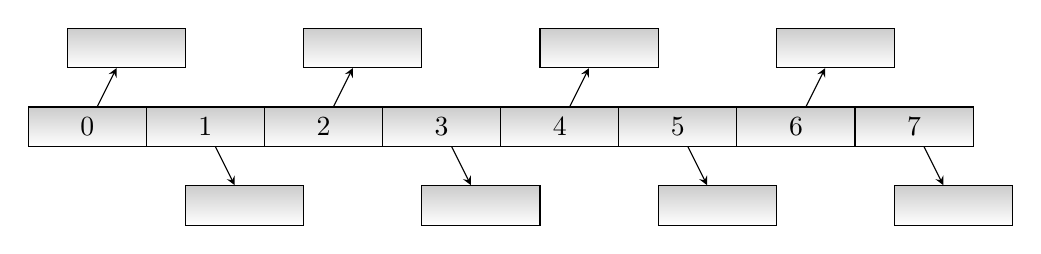
\begin{tikzpicture}
   [
      >=stealth,
      item/.style={rectangle, draw, inner sep=0pt, minimum width=1.5cm, minimum
      height=5mm, top color=black!20, bottom color=white}
   ]
   \foreach \i in {0,...,7}
      \node[item] (address\i) at (1.5*\i,1) {\i};

   \foreach \i in {0,2,...,6} {
      \node[item] (object\i) at (1.5*\i+0.5,2) {};
      \tikzmath{
         int \j;
         \j = \i+1;
      }
      \node[item] (object\j) at ({1.5*\j+0.5},0) {};
   }

   \foreach \i in {0,...,7}
      \draw[->] (address\i) -- (object\i);
\end{tikzpicture}
\end{document}

% vim: ft=tex tw=90 sts=-1 sw=3 et fdm=marker

   \captionsetup{width=.9\linewidth} % FIXME: hacks!
   \caption[Array of Pointers]{Array of Pointers; the array is compact but the actual
   objects may \alts{be scattered across memory pretty randomly, not be laid out
   sequentially in memory}.}
   \label{fig:true-oo}
\end{figure}

\subsubsection{Unrolled List}

% TODO.  Talk about unrolled lists and software prefetching.

% vim: tw=90 sts=-1 sw=3 et fdm=marker

% TODO: "Cache Replacement Policies", "Eviction (Policies|Strategies|Algorithms)" section?
% See <https://en.wikipedia.org/wiki/Cache_replacement_policies>.
\section{Abstract?}
% \section{Analysis of Algorithms}

% > However the efficiencies of any two "reasonable" implementations of a given algorithm
% > are related by a constant multiplicative factor called a *hidden constant*.
%      -- https://en.wikipedia.org/wiki/Analysis_of_algorithms

% Mathematical analysis of algorithms to obtain asymptotic upper bounds is nice.  Ignoring
% the non-uniform nature of memory hierarchies can yield pretty bad results, though.  What
% can be done about this?

We have seen that
\alts{
  {the hidden constant \alts{separating, distinguishing} the time complexities of two
  reasonable algorithms under asymptotic analysis can get quite big in the presence of a
  memory hierarchy.},
  {analyzing \alts{an algorithm's,} \alts{time, asymptotic, algorithmic} complexity,
  % This is not true: it doesn't matter for asymptotic complexity if there are different
  % types of memory.
  \x{under the usual \gls{ram} model, where a single uniform memory is \alts{presumed,
  assumed, supposed, premised},}
  can be quite inaccurate in the presence of a memory hierarchy.},
}
\alts{
  To \alts{escape, avert, prevent} having to rely \alts{only, entirely, exclusively} on
  empirical results, To overcome this problem,
},
abstract machine models taking the non-uniform \alts{memories of, nature of memory in}
real-world computers into account \alts{can be used, are used, have been proposed}.
% By whom?
One of these is the \emph{\gls{emm}}\x{\alts{
  ~\cite[5]{afmh},
  {, used \alts{in~\cite{afmh}, by \textcite{afmh}}.},
}}.

\subsection{External Memory Model}

% https://en.wikipedia.org/wiki/Random-access_machine

% TODO: go into more detail about the RAM model?
\alts[2]{
  {\alts{Establishing the basis of the, The} \gls{emm}, the widely used \gls{ram} model
  assumes \say{a \say{sufficiently} large uniform memory}~\cite[5]{afmh} with a constant
  access time.
  The},
  {The \gls{emm} is an extension of the \gls{ram} model.  While the latter assumes \say{a
  \say{sufficiently} large uniform memory}~\cite[5]{afmh} with a constant access time,
  the},
}
\gls{emm} \alts{divides, \alts{expands upon, extends} this by dividing} the memory into
\emph{internal} and \emph{external}.
\alts{The, Only the} internal memory is accessed directly, but its size is limited to
\(M\) \alts{items, words}.
The external memory is unbounded, but \alts{
  can only be accessed indirectly by loading data,
  data \x{is not accessed directly and} has to be loaded,
}
into internal memory \say{using \glslink{io}{I/Os} that move \(B\) contiguous
\alts{[items], words}}~\cite[5]{afmh}.

% > Although the word "I/O" suggests that external memory should be identified with disk
% > memory, we are free to choose any two levels of the memory hierarchy for internal and
% > external memory in the model.
%        -- Algorithms for Memory Hierarchies, page 6
The use of the term \emph{\acrshort{io}} here is somewhat non-standard.  While it suggests
\x{\alts{that, the}} external memory represents an \alts{
  {\gls{hdd} or \gls{ssd}},
  {\gls{hdd}, \gls{ssd} or similar},
}, it is
not constrained which \alts{physical storages, members of an actual memory hierarchy} are
\alts[2]{represented by, associated \alts{with, to}} \x{the} internal and external memory.
% Which members of an actual memory hierarchy are \alts{represented by, associated to} the
% internal and external memory is \alts{not constrained, as desired}.
If we choose the set of all CPU caches and the main memory, \(B\) becomes the cache line
size and \(M\) may be in the order of a few \si{\mebi\byte}.

The number of \acrshortpl{io} an algorithm requires in the \gls{emm} can augment the
information provided by standard asymptotic complexity analysis%
\x{, if \acrshort{io} is pivotal to an algorithm's runtime},
but \alts[2]{can't substitute, is no substitute for} measurements\x{~\cite[181]{afmh}}.
For example, the lower bound of \acrshortpl{io} needed for computing the sum of some
input of size \(N\), like in \cref{lst:ithare}, is
% See <http://erikdemaine.org/papers/BRICS2002/paper.pdf#page=7>.
\alts[3]{
  \(\lceil\nicefrac{N}{B}\rceil\),
  \(\left(\lfloor\nicefrac{N}{B}\rfloor + 2\right)\),
  \(\left(\lceil\nicefrac{N}{B}\rceil + 1\right)\),
}
in the \gls{emm}.\footnote{%
  TODO.
}
The linked list in that example probably takes almost \(N\) \acrshortpl{io},
though, since consecutive \alts{nodes, elements} are unlikely to fall into the same cache
line.  Thus, the predicted performance difference between \mintinline{cpp}{std::vector}
and \mintinline{cpp}{std::list} is at most \(B\), the number of items a cache line can
hold, which is \si{16} in this case.%
\footnote{%
  % TODO: elaborate on the size of `int`?
  A cache line is \alts{\si{64} bytes, \SI{64}{\byte}} on my laptop's CPU and an
  \mintinline{text}{int} \si{4} bytes with my compiler.
}
Recalling that the \alts{measured, actual} performance difference was
\num[round-mode=places, round-precision=0]{\speedup}, this is pretty inaccurate, but more
informative than saying both \x{algorithms'} data structure's time complexities for
traversal are \x{in} \(\Theta(N)\).

% An extensive repository of the theoretical lower bounds of \acrshortpl{io} needed in the
% \gls{emm} for many problems is available in the literature (for example \cite{afmh}).

Even with the simplifications made by the \gls{emm}, algorithmic analysis is usually only
done asymptotically: the number of \acrshortpl{io} is expressed \alts{in terms of, as}
\(\mathcal{O}\left(f\left(N, M, B\right)\right)\) or one of the related symbols.
Theoretical lower bounds of the \acrshortpl{io} needed in the \gls{emm} are available in
the literature (for example~\cite{afmh}) for many problems.

% This analysis only makes sense when \acrshort{io} is pivotal to an algorithm's
% efficiency.

% The objective is to \alts{
%   {design algorithms requiring a \alts{minimum number, minimum, minimal number} of
%   \acrshortpl{io}.},
%   {minimize the number of \alts{\acrshortpl{io}, I/Os} \alts{an algorithm needs,
%   needed}.},
% }

\x{
% Applying this model to \cref{lst:ithare} suggests
The \gls{emm} suggest that we can at best sum containers like in \cref{lst:ithare} using
\(\nicefrac{N}{B}\) \acrshortpl{io}, where \(N\) is the number of items to sum and \(B\)
the amount of them that fit in one block.
% Since there's 5000 containers of size 5000 and my cache line
% size is \SI{64}{B} and fits 8 \mintinline{cpp}{int} values:
% \begin{equation*}
%   N/B = 5000^2/8 = 3125000
% \end{equation*}
We can assume that the version with the list uses almost \(N\) \acrshortpl{io} because of
the random memory access.  Since a cache line fits 16 \mintinline{text}{int} values (\(B =
16\)) it
predicts a performance difference of 16.  This is not very accurate.
Analysis of \acrshortpl{io} needed by an algorithms \x{or data structure} may help inform
the decision of whether to consider it for empirical comparisons, though.
% that can be used prior to empirical comparisons.

% Apparently, the model is not practical for comparing these two data structures.
}

% Now for something completely different.
\x{
The \gls{emm} also suggests another approach to improve \cref{lst:ithare}, if we don't
want to \alts{trade, forgo, give up} the \x{asymptotically} constant time complexity of
insertions and deletions anywhere in the container: an \emph{unrolled list}.
}

% > In general it is best to hardcode cache line sizes at compile time by using the
% > `getconf` utility as in:
% >    gcc -DCLS=$(getconf LEVEL1_DCACHE_LINESIZE) ...
% > If the binaries are supposed to be generic, the largest cache line size should be
% > used.
%      -- Drepper, p. 50

% \subsubsection{Notes}
% \subsubsection{Caveats}
% \subsubsection{Limitations and Other Models}
\subsubsection{Limitations}

% Notes and potential problems:
% * The concept of I/Os that move B contiguous words directly translates to cache lines.
% * There's nothing equivalent to prefetching in the EMM.
% * > The main problem with hardware caches is that they use a fixed simplistic strategy
%   > for deciding which blocks are kept whereas the external memory model gives the
%   > programmer full control over the content of internal memory.
%        -- Algorithms for Memory Hierarchies, page 6
% * We lost associativity too.
% * And we don't model multiple levels of CPU caches, of course.

% Replacement policies.  Associativity.  More than two levels of memory.

% While the concept of \acrshortpl{io} directly models \alts{
%   most\footnote{%
%     TODO: not associativity though.
%   },
%   the
% }
% \alts{effects, existence} of cache lines,
% % are directly modeled by the concept of \acrshortpl{io},
% nothing in the \gls{emm} accounts for \x{those of} prefetching.

While the concept of \acrshortpl{io} directly models cache lines, most other
characteristics of memory hierarchies are ignored by the \gls{emm}.  For example:
\begin{itemize} % TODO: probably don't use a list structure.
  \item prefetching, or more generally the advantages of sequential access patterns,
  \item multi-level caches,
  \item the lack of direct control over the contents of caches, % (\alts{CPUs,
    % \glspl{cpu}} employ fixed, hardware-controlled replacement strategies)
  \item associativity,\footnote{%
      Associativity is not discussed in this paper; see \textcite{drepper2007} instead.
    }
  \item \gls{tlb}.
  % critical word stuff...
\end{itemize}
%
% > In the EMM it is generally assumed that the cost of I/Os is much greater than the cost
% > of computation, hence the design of the algorithm is usually motivated by the need to
% > minimise the number of I/Os.  However in the CMM and the IMM the relative miss
% > penalties are far smaller and we have to consider computation costs.
%      -- Algorithms for Memory Hierarchies, Section 8.6.4, page 188
%
% > The relative miss penalty is much lower for caches or the TLB than for disks, so
% > constant factors are important, we find that asymptotic analysis is not enough to
% > determine the performance of algorithms.
%      -- Algorithms for Memory Hierarchies, page 181
%
\alts{More fundamentally, Additionally}, the model's premise is that \acrshortpl{io} are
much more expensive than computation~\cite[188]{afmh}.
% This doesn't apply to data transfer between main memory and caches to the extent it does
% when accessing \glspl{hdd}.
While this is \alts{plausible, sensible, reasonable} when accessing \glspl{hdd}, it
doesn't apply to data transfer between main memory and caches to nearly the same extent.
%
Some of these shortcomings are addressed by refined machine models, which include more
details of real caches~\cite[178]{afmh}.
% I.e., CMM (cache memory model) and IMM (internal memory model).  There doesn't seem to
% be much literature about them [1].  Algorithms for Memory Hierarchies only cites a
% single paper that uses the IMM.  Don't discuss them.
%
% [1]: https://www.google.com/search?q=cache+memory+model+cmm
This complicates mathematical analysis~\cite[181]{afmh} and heuristics may be
used~\cite[191]{afmh}, which in turn \alts{exacerbates, amplifies} the need for
accompanying measurements~\cite[181]{afmh}.

\x{
\alts{
  {\alts[2]{On the contrary, Contrarily}, the \emph{\gls{com}} further increases the level
  of abstraction},
  {The opposite approach -- towards more abstraction -- is taken by the \gls{com}},
}.
}

% CMM and IMM add more detail ... bla bla bla ... COM actually abstracts further ...  bla
% bla ... counterintuitively this makes it more fitting in one aspect ... it works across
% the whole memory hierarchy ...

% vim: tw=90 sts=-1 sw=3 et fdm=marker

\subsection{Cache-Oblivious Model}
%           Model-Oblivious Algorithms
%           Ideal-Cache Model
%           \Gls{com}

% This one's kind of nice (and Scott Meyers seems to think it has merit).  It also has a
% Wikipedia page, unlike the EMM, CMM, or IMM (a very rough index of practicality).

% This seems like FUD:
%
% > Typical cache-efficient algorithms require tuning to several cache parameters which
% > are not always available from the manufacturer and often difficult to extract
% > automatically.
%      -- http://erikdemaine.org/papers/BRICS2002/paper.pdf

% > In computing, a cache-oblivious algorithm (or cache-transcendent algorithm) is an
% > algorithm designed to take advantage of a CPU cache without having the size of the
% > cache (or the length of the cache lines, etc.) as an explicit parameter.
%      -- https://en.wikipedia.org/wiki/Cache-oblivious_algorithm
%

The \emph{\gls{com}} or \emph{ideal-cache model}, introduced by
\textcite{coa-for-publication}, \alts{concedes, leaves, forfeits} most of the
aforementioned problems to empirical evaluation and further increases the level of
abstraction.
%
Algorithms for the \gls{com}, called \emph{cache-oblivious algorithms}, are designed
without the \alts{
  cache size \(M\) or block size \(B\),
  values of \(M\) and \(B\),
}
as parameters.  This seems silly since these values typically can be queried easily
\x{automatically} at both run and compile time~\cite[50]{drepper2007}
% See <https://stackoverflow.com/a/7284876>.  Also, cache line sizes are super homogeneous
% anyway.
but, perhaps counterintuitively, models one aspect of memory hierarchies better than the
\gls{emm}.
% > This model was born out of the necessity to capture the hierarchical nature of memory
% > organization. [...] Although there have been other attempts to capture this
% > hierarchical information the cache oblivious model seems to be one of the most simple
% > and elegant ones.
%      -- Algorithms for Memory Hierarchies, page 194
%
% > The ideal cache oblivious model enables us to reason about a two level memory like the
% > external memory model but prove results about a multi-level memory model.
%      -- Algorithms for Memory Hierarchies, page 195
%
% > One consequence is that, if a cache-oblivious algorithm performs well between two
% > levels of the memory hierarchy (nominally called cache and disk), then it must
% > automatically work well between any two adjacent levels of the memory hierarchy.
%      -- http://erikdemaine.org/papers/BRICS2002/paper.pdf (erikcom)
%
% > Good algorithms for this model give us good algorithms for all values of B and M.
% > They are especially useful for multi-level caches.
%      -- https://ocw.mit.edu/courses/electrical-engineering-and-computer-science/6-851-advanced-data-structures-spring-2012/calendar-and-notes/MIT6_851S12_L7.pdf
%
% > From a theoretical standpoint, the cache-oblivious model is appealing because it is
% > very clean.  A cache-oblivious algorithm is simply a RAM algorithm; it is only the
% > analysis that differs.  The cache-oblivious model also works well for multilevel
% > memory hierarchies, unlike the external-memory model, which only captures a two-level
% > hierarchy.
%      -- https://pdfs.semanticscholar.org/2f5a/76ccdc71971b746fbe7ff54db86c65a73e91.pdf
%
% > Frigo et al. showed that for many problems, an optimal cache-oblivious algorithm will
% > also be optimal for a machine with more than two memory hierarchy levels.
%      -- https://en.wikipedia.org/wiki/Cache-oblivious_algorithm
%
% > [W]e prove that an optimal cache-oblivious algorithm designed for two levels of memory
% > is also optimal for multiple levels.  We also prove that any optimal cache-oblivious
% > algorithm is also optimal in the previously studied HMM and SUMH models.
%      -- https://pdfs.semanticscholar.org/19ed/9795adc7204d3c9745b3c9f71f8496d26bb6.pdf
%
% > We prove that an optimal cache-oblivious algorithm designed for two levels of memory
% > is also optimal for multiple levels and that the assumption of optimal replacement in
% > the ideal-cache model can be simulated efficiently by LRU replacement.
%      -- http://supertech.csail.mit.edu/papers/FrigoLePr99.pdf#page=1, Abstract
%
An algorithm that performs well in the \gls{com} performs well across the entire memory
hierarchy~\cites[194\psq]{afmh}[4]{erikcom}; the same argument \alts[2]{\alts{for,
showing} asymptotically optimal movement of data, for data movement being
\x{asymptotically} \emph{optimal}} applies between any two levels of memory%
~\cite[lemma 15, \pno~10]{coa-paper}.
% TODO.  Is asymptotic analysis even useful, though?  The whole point of these models is
% that the hidden constants of "standard" asymptotic analysis matter.

% What does "optimal" mean?
%
% > An optimal cache-oblivious algorithm is a cache-oblivious algorithm that uses the
% > cache optimally (in an asymptotic sense, ignoring constant factors).
%      -- https://en.wikipedia.org/wiki/Cache-oblivious_algorithm
%
% > We say that [an algorithm] is *cache optimal* if the number of cache misses meet the
% > asymptotic lower bound for I/Os in the EMM for that problem.
%      -- Algorithms for Memory Hierarchies, page 181
%
% > [T]hese algorithms use an optimal amount of work and move data optimally among
% > multiple levels of cache.
%      -- http://supertech.csail.mit.edu/papers/FrigoLePr99.pdf#page=1, Abstract
%
% > For simplicity in this paper, we use the term "optimal" as a synonym for
% > "asymptotically optimal", since all our analyses are asymptotic.
%      -- http://supertech.csail.mit.edu/papers/FrigoLePr99.pdf#page=2, footnote
Optimal means that the asymptotic~\cite[2]{coa-paper} number of cache misses incurred
\x{by a cache-oblivious algorithm} matches the problem's lower bound in the \gls{com}.

% > In contrast to the external-memory model, algorithms in the cache-oblivious model
% > cannot explicitly manage the cache (issue block-read and block-write requests).  This
% > loss of freedom is necessary because the block and cache sizes are unknown.
%      -- http://erikdemaine.org/papers/BRICS2002/paper.pdf (erikcom), page 5
Cache misses take the place of \acrshortpl{io} \x{used in the \gls{emm}} because
cache-oblivious algorithms don't \alts{manage the cache, read or write cache lines}
explicitly.  This wouldn't be possible since the algorithms know neither the cache nor
the cache line size~\cite[5]{erikcom}.
% > The ideal cache uses the optimal off-line strategy of replacing the cache line whose
% > next access is furthest in the future
%      -- http://supertech.csail.mit.edu/papers/FrigoLePr99.pdf#page=1
Instead, the \gls{com} uses the optimal replacement strategy of evicting the cache line
that won't be accessed for the longest time in the future (Bélády's Algorithm).  This
\alts{
  is strangely \alts{at odds, out of touch, unrealistic} with real-world caches that don't
  know the future,
  {seems like out-of-touch, theoretical ivory-tower nonsense},
}.
% > The ideal-cache model makes the perhaps-questionable assumptions that there are only
% > two levels in the memory hierarchy, that memory is managed automatically by an optimal
% > cache-replacement strategy, and that the cache is fully associative.  We address these
% > assumptions in Section 6, showing that to a certain extent, these assumptions entail
% > no loss of generality.
%      -- http://supertech.csail.mit.edu/papers/FrigoLePr99.pdf#page=2
%
% > LRU and FIFO replacement do just as well as optimal replacement up to a constant
% > factor of memory transfers and up a constant factor wastage of the cache.
%      -- http://erikdemaine.org/papers/BRICS2002/paper.pdf#page=6 (erikcom)
%
% > The same argument extends to a variety of other replacement strategies.
%      -- http://supertech.csail.mit.edu/papers/Prokop99.pdf#page=46
%
% > We show that algorithms with regular complexity bounds (Equation (7.1)) (including all
% > algorithms heretofore presented) can be ported to less-ideal caches incorporating
% > least-recently-used (LRU) or first-in, first-out (FIFO) replacement policies [24, p.
% > 378].
%      -- http://supertech.csail.mit.edu/papers/Prokop99.pdf#page=51
%
% > [I]n many cases [the COM] is provably within a constant factor of a more realistic
% > cache's performance.
%      -- https://en.wikipedia.org/wiki/Cache-oblivious_algorithm
%
% > [A]s long as the number of memory transfers depends polynomially on the cache size M,
% > then halving M will only affect the running time by a constant factor.
%      -- http://erikdemaine.org/papers/BRICS2002/paper.pdf#page=6 (erikcom)
%
% > Intuitively, algorithms that slow down by a constant factor when memory (M) is reduced
% > to half, are called regular.
%      -- Algorithms for Memory Hierarchies, page 196
However, \citeauthor{coa-thesis} proves that for many algorithms\footnote{%
   Those satisfying equation (7.1) in~\cite[46]{coa-thesis}.  If the number of cache
   misses incurred by the algorithm only \say{depends polynomially on the cache size
   \(M\)}, the \alts{equation, condition} is satisfied~\cite[6]{erikcom}.
   % Halving the cache size only increases the number of cache misses by a constant
   % factor?
}
it only increases cache misses by a constant factor compared to various feasible
replacement strategies%
% ~\cite[lemma 12, \pno~10]{coa-paper}.%
% ~\cite[corollary 13, \pno~10]{coa-paper}.%
~\cite[corollary 19, \pno~46]{coa-thesis}.%
% See <http://supertech.csail.mit.edu/papers/Prokop99.pdf#page=46>.
\footnote{%
   e.g. LRU, FIFO, and random replacement
}

% According to `coa-paper` (page 9), the "four major assumptions" are:
% *  automatic replacement
% *  optimal replacement
% *  two levels of memory
% *  full associativity
%
% All simplifications and assumptions (I think):
% *  inherited/adopted from the EMM
%    *  two levels of memory
%    *  full associativity
%    *  tall cache
%       *  "It is also commonly assumed in external-memory algorithms."
%             -- http://erikdemaine.org/papers/BRICS2002/paper.pdf#page=7
%       *  I don't grok this one.
% *  new
%    *  automatic, optimal replacement
%    *  inclusion property
%       *  "[T]he values stored in cache i are also stored in cache i+1"
%             -- http://supertech.csail.mit.edu/papers/FrigoLePr99.pdf#page=10
%
% TODO: reiterate all simplifications and assumptions?

% > We show that the assumptions of two hierarchical memory models in the literature, in
% > which memory movement is programmed explicitly, are actually no weaker than ours.
% > Specifically, we prove (with only minor assumptions) that optimal cache-oblivious
% > algorithms in the ideal-cache model are also optimal in the hierarchical memory model
% > (HMM) [1] and in the serial uniform memory hierarchy (SUMH) model [5, 42].
%      -- http://supertech.csail.mit.edu/papers/Prokop99.pdf#page=12
%
% Exactly the same text is in the paper.  But only in the earlier version [1].
% [1]: https://pdfs.semanticscholar.org/19ed/9795adc7204d3c9745b3c9f71f8496d26bb6.pdf
%
% > An optimal cache-oblivious algorithm whose cache-complexity bound satisfies the
% > regularity condition (14) can be implemented optimally in expectation in multilevel
% > models with explicit memory management.
%      -- http://supertech.csail.mit.edu/papers/FrigoLePr99.pdf#page=11, theorem 17
%
% > [W]e have shown that optimal cache-oblivious algorithms in the ideal-cache model are
% > also optimal in the hierarchical memory model (HMM).
%      -- http://supertech.csail.mit.edu/papers/Prokop99.pdf#page=56
%
\citeauthor{coa-thesis} further justifies the model by proving, \say{with only minor
assumptions}~\cite[12]{coa-thesis}, that cache-oblivious algorithms that are optimal in
the \gls{com} \alts{can by executed with an optimal amount of \acrshortpl{io}, are also
optimal} in the \gls{emm}~\cite[theorem 32, \pno~56]{coa-thesis}.  In other words, most
cache-oblivious algorithms can be systematically transformed into \alts{cache-aware,
\gls{emm}} algorithms that asymptotically require the same amount of memory transfers in
the \gls{emm} as the cache-oblivious variant in the \gls{com}.

% TODO: given our motivation that "constant factors matter", what have we been doing here?

% TODO.  A regular algorithm that isn't explicitly for a hierarchical memory model
% (doesn't explicitly move data between different levels of memory) is already
% cache-oblivious, right?

% Time to give an example algorithm.  Options:
% *  matrix transposition
% *  matrix multiplication
% *  searching a tree (Van Emde Boas layout vs. standard layout)
% *  sorting
%    *  not easy
%    *  good performance seems problematic
%    *  looks like the autors of [1] dit it, though (lazy funnelsort)
% *  something about linked lists?
%
% Maybe matrix transposition...
%
% [1] https://app.cs.amherst.edu/~ccmcgeoch/cs34/papers/a2_2-brodal.pdf
\subsubsection{Cache-Oblivious Matrix Transposition}

The straightforward way to transpose \alts{
   an \(m\times n\) matrix \(D\),
   a matrix \(D\in\mathbb{R}^{m\times{}n}\),
}
out-of-place is to use two loops like so:
\begin{minted}[autogobble]{c}
   for (int i = 0; i < m; ++i)
      for (int j = 0; j < n; ++j)
         E[j][i] = D[i][j];
\end{minted}
Assuming \(D\) and \(E\) are stored in row-major layout (as they would be in the C and
\cpp{} languages), the reads from \(D\) are sequential memory accesses but the writes to
\(E\) are not.

\alts{When \(D^\mathsf{T}\) has, For} sufficiently long rows (\(m > B\))\footnote{%
   \(D^\mathsf{T}\) will be an \(n\times m\) matrix, so \(m\) is its number of columns.
},
every consecutive access will be to a different cache line.  If it has sufficiently many
rows, no access will be to a cache line that is still loaded; once the inner loop
completes, the cache line holding \alts[2]{\mintinline{c}{E[0][i]}, \(B_{0,i}\)} will have
been evicted.%
\footnote{%
   assuming LRU or FIFO replacement % FIXME: but we use optimal replacement!
}
Therefore, this algorithm incurs \(\Theta(mn)\) cache misses.

The algorithm is \alts{by definition, technically} already cache-oblivious since it
doesn't use \(M\) or \(B\), but it is not optimal\x{ in the \gls{com}}.  We can do better
with a divide-and-conquer approach.
% The code may only be 72 characters wide (75 when counting the indentation that will be
% stripped).  Note that the array arguments will decay to pointers.
\begin{minted}[autogobble, mathescape]{c}
   // Transpose the submatrix $(d_{ij})_{i\in I,\:j\in J}$.
   void transpose(int I[2], int J[2], int D[m][n], int E[n][m]) {
      int num_rows = 1 + I[1] - I[0];
      int num_cols = 1 + J[1] - J[0];
      if (num_cols == 1 && num_rows == 1) {
         E[J[0]][I[0]] = D[I[0]][J[0]];
      } else if (num_cols <= num_rows) {
         // Horizontally slice D into two submatrices and recurse.
         transpose((int[2]){I[0], I[0] + num_rows / 2 - 1}, J, D, E);
         transpose((int[2]){I[0] + num_rows / 2, I[1]}, J, D, E);
      } else { /* Vertically slice D analogously... */ }
   }
\end{minted}
% // Transpose the submatrix $(d_{ij}),\: i\in I, j\in J$.
% // Transpose the submatrix $(d_{ij})_{I_0<i<I_1, J_0<j<J_1}$
% // Transpose the submatrix $D\left[...\right]$

\begin{figure}
   \centering
   \begin{tikzpicture}
      \datavisualization
      [scientific axes=clean,
       x axis={logarithmic,
               label={Matrix Size (\si{\mebi\byte})}, length=0.8\textwidth, ticks={
                  major at={1, 2, 4, 8, 16, 32, 64, 128, 256},
               },
              },
       y axis={include value=0, grid=at ticks, label={Speedup}, length=6cm,
         % ticks={major also at={1}}
       },
       visualize as scatter,
       scatter={style={mark=*, mark options={scale=.65}}}]
         data [read from file=xpose/speedup.csv, separator=\space];
   \end{tikzpicture}
   \caption{TODO}
   \label{fig:TODO}
\end{figure}

% > A cache-oblivious algorithm is simply a RAM algorithm; it is only the analysis that
% > differs.
%      -- https://pdfs.semanticscholar.org/2f5a/76ccdc71971b746fbe7ff54db86c65a73e91.pdf
%
% Algorithms are cache-oblivious by default.

% Work by Erik Demaine:
%
% [1]: http://erikdemaine.org/papers/BRICS2002/paper.pdf
%      "Cache-Oblivious Algorithms and Data Structures - 2002"
% [2]: https://web.archive.org/web/20160320051801/http://courses.csail.mit.edu/6.897/spring03/scribe_notes/L15/lecture15.pdf
%      "6.897: Advanced Data Structures - Spring 2003"
% [3]: https://pdfs.semanticscholar.org/2f5a/76ccdc71971b746fbe7ff54db86c65a73e91.pdf
%      "6.897: Advanced Data Structures - Spring 2005"
% [4]: https://ocw.mit.edu/courses/electrical-engineering-and-computer-science/6-851-advanced-data-structures-spring-2012/calendar-and-notes/MIT6_851S12_L7.pdf
%      "6.851: Advanced Data Structures - Spring 2012"

% vim: tw=90 sts=-1 sw=3 et fdm=marker


% [1]: https://en.wikipedia.org/wiki/Analysis_of_algorithms

% vim: tw=90 sts=-1 sw=3 et fdm=marker

% \section{Parallel Computing}

\subsection{Cache Coherence}
%           Cache Coherency

% https://en.wikipedia.org/wiki/Cache_coherence

% Dirty.
% Invalid.

% vim: tw=90 sts=-1 sw=3 et fdm=marker

% % \subsection{False Sharing}
\section{False Sharing}

% vim: tw=90 sts=-1 sw=3 et fdm=marker

% TODO: "Roofline" section?  See <https://en.wikipedia.org/wiki/Roofline_model>.

\clearpage
\begin{appendices} % <https://tex.stackexchange.com/q/49643>
   \crefalias{section}{appsec} % See <https://tex.stackexchange.com/q/119513>.
   \crefalias{subsection}{appsec}
   \section{Reading Information About the CPU}
\label{app:cpuinfo}
% https://stackoverflow.com/q/7281699
% https://unix.stackexchange.com/q/167038
% https://superuser.com/q/55776
There are many ways to display information about the processor(s) the operating system is
running on.  Among others, the \mintinline{text}{lscpu(1)} and
\mintinline{text}{getconf(1)} programs and the \mintinline{text}{/proc/cpuinfo}
pseudo-file on Linux.  This is how I checked my CPU's cache sizes, for example:
\begin{minted}[gobble=3]{bash}
   $ lscpu | grep 'L1d\|L2'
   L1d cache:             32K
   L2 cache:              512K
\end{minted}
%stopzone
This is what I used to get the cache line sizes:
\begin{minted}[gobble=3]{bash}
   $ getconf LEVEL1_DCACHE_LINESIZE; getconf LEVEL2_CACHE_LINESIZE
   64
   64
\end{minted}
%stopzone

% vim: tw=90 sts=-1 sw=3 et fdm=marker

   % Performance Analysis; Run Time Analysis; Timing Methodology; Profiling Pitfalls; Run
% Time Measuring; Benchmarking Methodology; Performance Monitoring
\section{Profiling Methodology}
\label{app:meth}

% Programs: `time`, bad; `\time -v`, better; oprofile(1); gprof(1); perf; Valgrind's
% cachegrind?; ...

\begin{comment}
Plenty of things can go wrong when \alts{profiling, measuring \alts{execution, run}
times}.  These are the ones I was aware of and tried to account for while doing
measurements for this \article.
\begin{itemize}
   \item \emph{CPU frequency scaling and boosting}.
      CPU frequencies are usually dynamic these days and automatically adjusted based on
      at least workload and temperature.  This should be disabled when measuring execution
      times.  I used the cpupower(1) program.
      % See <https://wiki.archlinux.org/index.php/CPU_frequency_scaling> and
      % <https://github.com/torvalds/linux/tree/master/tools/power/cpupower>.
      \begin{minted}[autogobble]{text}
         # cpupower frequency-set -g performance
         $ ./benchmark
         # cpupower frequency-set -g schedutil
      \end{minted}
      %stopzone
      % See [5].  Not a problem when measuring cycles.
   \item \emph{Interrupts and context switches.}  The process being timed has to share
      resources with other processes and the operating system.  A context switch will not
      only increase wall time, it will also increase cycles because of TLB flushes and
      cache evictions. % See <https://en.wikipedia.org/wiki/Context_switch>.

      Processor shielding, % See [5].
      taking the minimum of several measurements, and assigning a very high priority can
      \alts{help here, mitigate these problems}.
      % This is likely better than using nice(1).
      \begin{minted}[autogobble]{text}
         # chrt -f 99 \time -v ./program
      \end{minted}
   \item \emph{CPU jumping.}
      % See <https://youtu.be/vrfYLlR8X8k?t=33m34s>.
      CPU pinning (setting processor/thread affinity) may help. % See [2] and [5].
   \item \emph{Cache warmth.}
      % See <https://youtu.be/vrfYLlR8X8k?t=41m00s>.
      When comparing different solutions on the same data set, later ones may benefit from 
      data having been loaded into cache already.  Checking whether swapping the order of
      measurements changes the results is a good idea.
\end{itemize}
These effects may \alts{add noise to, pollute} the results, render them irreproducible, or
invalidate them completely.

General mitigation/alleviation strategy: take the minimum execution time of \alts{all, a
number of} runs; all noise is additive (TODO: not the one caused by the cache being hot).
% See [7].
\end{comment}

All programs were compiled and run on Linux using the \gls{gcc} with
\mintinline{text}{-O2} (unless noted otherwise) and \mintinline{text}{-march=native}.
% Additionally,
I disabled CPU frequency scaling with \mintinline{text}{cpupower(1)},
% See <https://wiki.archlinux.org/index.php/CPU_frequency_scaling>.
reduced the number of running processes,%
\footnote{%
   I stopped Firefox (which added visible noise) and the X server, for example.
}
% (e.g. leaving Firefox open in the background added lots of noise),
and assigned a high priority to the benchmark process with the \mintinline{text}{chrt(1)}
command.

The \emph{\href{https://github.com/meribold/cache-seminar-paper/blob/master/makefile}
{makefile}} used to compile and run the measurements as well as the full source code of
the programs is available \alts{at, here:, on GitHub:}
\url{https://github.com/meribold/cache-seminar-paper}.

\subsection{Measuring CPU cycles}
\label{app:cycles}

% Frequency scaling is still a problem here.  For example, when the program is memory
% bound, it may take fewer cycles at a lower frequency while completing in the same wall
% time.  I.e., not everything is proportional to CPU frequency.

% > OProfile leverages the hardware performance counters of the CPU.
%      -- http://oprofile.sourceforge.net/about/

% > `ocount` is an OProfile tool that can be used to count native hardware events
% > occurring in [...] a specific application.
%      -- http://oprofile.sourceforge.net/doc/getting-started-with-ocount.html

% A list of AMD family 14h CPU performance counters is available at [1].  `ophelp(1)` can
% also be used.
% [1]: http://oprofile.sourceforge.net/docs/amd-family14h-events.php

I used the \mintinline{text}{ocount(1)} event counting tool added to the
\citetitle{oprofile}~\cite{oprofile} project in version 0.9.9.
% `perf(1)` seems to be a newer alternative to OProfile [8].  TODO: use it?
%
% > Newer CPU models support a hardware performance counter mode which uses hardware logic
% > to record events without any active code needed
%      -- https://en.wikipedia.org/wiki/OProfile
It uses \emph{hardware performance counters}%
\footnote{%
   \url{https://en.wikipedia.org/wiki/Hardware_performance_counter}
}
to provide low-overhead performance information without source code modifications.
\alts{%
   {Essentially, this is the procedure:},
   The \x{exact} process is more or less
}

% diff <(gcc -march=native -E -v - </dev/null 2>&1) <(gcc -E -v - </dev/null 2>&1)
% gcc -O2 -fno-prefetch-loop-arrays -Q --help=optimizers

\begin{minted}[autogobble]{text}
   $ gcc -march=native -O2 program.c
   # cpupower frequency-set -g performance
   # chrt -f 99 ocount -e CPU_CLK_UNHALTED ./a.out
\end{minted}
%stopzone

% ~\cite[78\psqq]{drepper2007}.

% [1]: https://en.wikipedia.org/wiki/Profiling_(computer_programming)
% [2]: https://en.wikipedia.org/wiki/Processor_affinity
% [3]: https://en.wikipedia.org/wiki/OProfile
% [4]: https://en.wikipedia.org/wiki/Perf_(Linux)
% [5]: https://github.com/JuliaCI/BenchmarkTools.jl/blob/master/doc/linuxtips.md
% [6]: http://stackoverflow.com/q/9006596 "On `/usr/bin/time` for benchmarks and `perf`"
% [7]: https://youtu.be/vrfYLlR8X8k "Andrei Alexandrescu - Writing Fast Code"
% [8]: http://oprofile-list.sf.narkive.com/rVbJlHdX/oprofile-vs-perf
% [9]: https://serverfault.com/q/161008
%      "What is the difference between renice and chrt commands in Linux?"

% vim: tw=90 sts=-1 sw=3 et fdm=marker

   \section{Amazing Data}
\label{app:data}

\begin{center}
   \pgfplotstabletypeset[
      % See <https://tex.stackexchange.com/q/131081/#comment311347_137554>.
      assign column name/.code=\pgfkeyssetvalue{/pgfplots/table/column name}{{{#1}}},
      every head row/.style={%
         before row=\toprule,
         % output empty row,
         % before row={%
         %    \\\toprule
         %    Array Sizes (KiB) & \multicolumn{2}{c}{Cycles / Iteration} \\
         % },
         after row=\midrule,
      },
      every last row/.style={%
         after row=\bottomrule,
      },
      columns={x, y, x, y},
      columns/x/.style={
         assign column name={Array Size (KiB)},
         numeric as string type,
         % Using `divide by=1024` or `preproc/expr={##1/1024}` performs floating-point
         % math and introduces errors.  This abomination hacked together by trial and
         % error doesn't.
         preproc cell content/.code={%
            \pgfkeysgetvalue{/pgfplots/table/@cell content}\a
            \newcount\b
            \b=\number\a
            \divide\b by 1024
            \pgfkeyssetvalue{/pgfplots/table/@cell content}{\the\b}
         },
      },
      columns/y/.style={
         assign column name={Cycles / Iteration},
         string type,
         column type={S[round-mode=places, round-precision=2]},
         % column type=c, dec sep align,
         % fixed, fixed zerofill, precision=3,
      },
      % Split the table into two (super?) columns.  See page 42 and 43 of the
      % pgfplotstable manual.
      display columns/0/.style={
         select equal part entry of={0}{2},
         column type={S[table-format=3.0]},
      },
      display columns/1/.style={select equal part entry of={0}{2}},
      display columns/2/.style={
         select equal part entry of={1}{2},
         column type={S[table-format=6.0]},
      },
      display columns/3/.style={select equal part entry of={1}{2}},
   ]{access-times/access-times.csv}
   \captionof{table}{Access Times for Random Reads}
   \label{tab:access-times}
\end{center}

% FIXME: DRY!
\begin{center}
   \pgfplotstabletypeset[
      assign column name/.code=\pgfkeyssetvalue{/pgfplots/table/column name}{{{#1}}},
      every head row/.style={%
         before row=\toprule,
         after row=\midrule,
      },
      every last row/.style={%
         after row=\bottomrule,
      },
      columns={x, y, x, y},
      columns/x/.style={
         assign column name={Array Size (KiB)},
         numeric as string type,
         preproc cell content/.code={%
            \pgfkeysgetvalue{/pgfplots/table/@cell content}\a
            \newcount\b
            \b=\number\a
            \divide\b by 1024
            \pgfkeyssetvalue{/pgfplots/table/@cell content}{\the\b}
         },
      },
      columns/y/.style={
         assign column name={Cycles / Iteration},
         string type,
         column type={S[round-mode=places, round-precision=2]},
      },
      display columns/0/.style={
         select equal part entry of={0}{2},
         column type={S[table-format=3.0]},
      },
      display columns/1/.style={select equal part entry of={0}{2}},
      display columns/2/.style={
         select equal part entry of={1}{2},
         column type={S[table-format=6.0]},
      },
      display columns/3/.style={select equal part entry of={1}{2}},
   ]{seq-access-times/access-times.csv}
   \captionof{table}{Access Times for Sequential Reads}
   \label{tab:seq-access-times}
\end{center}

% vim: tw=90 sts=-1 sw=3 et fdm=marker

   % \section{Disabling the Prefetcher}
My initial results from from running \cref{lst:array-sum} were quite different.  See TODO.

TODO: I installed \texttt{msr-tools} and OProfile.
% This seems to work.  It did affect performance.  See
% <https://community.amd.com/thread/180725>.
\begin{minted}[gobble=3]{bash}
   $ sudo modprobe msr
   $ sudo rdmsr -a 0xC0011022
   600001800000000
   600001800000000
   $ sudo wrmsr -a 0xC0011022 0x600001800002000
   $ sudo rdmsr -a -f '13:13' 0xC0011022
   1
   1
   $ sudo rdmsr -a 0xC0011022
   600001800002000
   600001800002000
   $ sudo ocount -e PREFETCH_INSTRUCTIONS_DISPATCHED ./a.out
\end{minted}
%stopzone
I think resetting the MSR to enable hardware prefetches doesn't work.  To get the same
benchmmark results as before tweaking it, I have to reboot.

% vim: tw=90 sts=-1 sw=3 et fdm=marker

\end{appendices}

\clearpage

\printglossary[type=\acronymtype] % Print the list of acronyms.

\printbibliography[heading=bibintoc]

\end{document}

% vim: tw=90 sts=-1 sw=3 et fdm=marker
